\documentclass[11pt,a4paper]{article}
\usepackage[T1]{fontenc}
\usepackage{lmodern,microtype}
\usepackage{amsmath,amssymb,amsthm,array,geometry,booktabs,xcolor,graphicx,hyperref}
\geometry{margin=2.4cm}
\hypersetup{colorlinks=true,linkcolor=blue!60!black,urlcolor=blue!60!black,citecolor=blue!60!black,
pdftitle={Logical resource estimates for optimal execution by Cole-Hopf linearisation and Schroedingerisation},
pdfauthor={Xavier Bergeron}}
\graphicspath{{figures/}{../simulation/figures/}}
\newtheorem{proposition}{Proposition}
\newtheorem{lemma}[proposition]{Lemma}
\newtheorem{theorem}[proposition]{Theorem}
\theoremstyle{remark}
\newtheorem{remark}[proposition]{Remark}
\newcommand{\x}{\mathbf x}
\newcommand{\X}{\mathbf X}
\newcommand{\vv}{\mathbf v}
\newcommand{\Hd}{\hat H_d}
\newcommand{\eps}{\varepsilon}
\newcommand{\Psucc}{P_{\rm succ}}
\newcommand{\tr}{\operatorname{tr}}
\DeclareUrlCommand\lean{\urlstyle{tt}}
\makeatletter\@beginparpenalty=10000\makeatother % keep a heading with its list
% Written by simulation/make_numbers.py; do not edit.
\newcommand{\TAFive}{1.4\times10^{12}}
\newcommand{\TAsingleFive}{1.2\times10^{11}}
\newcommand{\QAFive}{161}
\newcommand{\TBFive}{1.5\times10^{10}}
\newcommand{\QBFive}{137}
\newcommand{\TAOne}{1.1\times10^{14}}
\newcommand{\TAsingleOne}{1.0\times10^{13}}
\newcommand{\QAOne}{186}
\newcommand{\TBOne}{2.2\times10^{12}}
\newcommand{\QBOne}{160}
\newcommand{\TATenth}{1.9\times10^{17}}
\newcommand{\TAsingleTenth}{1.8\times10^{16}}
\newcommand{\QATenth}{231}
\newcommand{\TBTenth}{8.6\times10^{15}}
\newcommand{\QBTenth}{187}
\newcommand{\RatioAB}{52}
\newcommand{\RatioABSingle}{4.7}
\newcommand{\StepsA}{3512}
\newcommand{\StepsB}{1812}
\newcommand{\ReadoutRuns}{7.9\times10^{5}}
\newcommand{\RunsBOne}{4.6\times10^{5}}
\newcommand{\OracleShareA}{83}
\newcommand{\PrepShareA}{0.5}
\newcommand{\SerialDaysB}{25}
\newcommand{\SerialYearsA}{3.5}
\newcommand{\OracleMin}{73}
\newcommand{\OracleMax}{85}
\newcommand{\KappaB}{3.88}
\newcommand{\TableA}{%
$\nu$ & 8 & 16 & 8\\
grid $N\times N$; $\Delta x$ & $32^2$; 1.000 & $64^2$; 0.667 & $256^2$; 0.121\\
readout span $h$ & 4 & 8 & 16\\
$p$-profile; $\eta_{\max}$; $n_p$ & $g_1$; 10; 9 & $g_1$; 20; 12 & $g_2$; 20; 15\\
grid error charged (measured) & $1.4\times10^{-2}$ ($6.9\times10^{-3}$) & $2.9\times10^{-3}$ ($1.7\times10^{-3}$) & $3.8\times10^{-4}$ ($1.2\times10^{-4}$)\\
LCU normalisation $\alpha$ & 45 & 155 & 2190\\
$P_{\rm succ}$ & 0.41 & 0.35 & 0.16\\
walk steps per run (standard QSP) & 641 (1228) & 3512 (6952) & 44907 (89724)\\
T per walk step (potential oracle) & 2925 (2420) & 3635 (3028) & 5200 (4428)\\
T per coherent run & $1.9\times10^{6}$ & $1.3\times10^{7}$ & $2.3\times10^{8}$\\
$\log_2M_j$, four amplitudes & 14, 12, 13, 12 & 17, 16, 17, 16 & 24, 22, 23, 23\\
coherent runs per estimate set & $6.6\times10^{4}$ & $7.9\times10^{5}$ & $7.5\times10^{7}$\\
total T, one estimate set & $1.2\times10^{11}$ & $1.0\times10^{13}$ & $1.8\times10^{16}$\\
\textbf{total T, median of 11} & $\mathbf{1.4\times10^{12}}$ & $\mathbf{1.1\times10^{14}}$ & $\mathbf{1.9\times10^{17}}$\\
\textbf{logical qubits} & \textbf{161} & \textbf{186} & \textbf{231}\\}
\newcommand{\TableB}{%
grid $N\times N$; half-width $L/\sqrt\nu$ & $32^2$; 5 & $64^2$; 5.5 & $128^2$; 6\\
$p$-profile; $\eta_{\max}$; $n_p$ & $g_{1/2}$; 5; 8 & $g_{1/2}$; 10; 10 & $g_{1/2}$; 40; 14\\
systematic error $r$ & $1.3\times10^{-2}$ & $2.2\times10^{-3}$ & $4.8\times10^{-4}$\\
LCU normalisation $\alpha$ & 51 & 148 & 470\\
$P_{\rm succ}$ & 0.65 & 0.56 & 0.43\\
walk steps per run & 428 & 1812 & 19672\\
T per walk step (potential oracle) & 1982 (1444) & 2541 (1920) & 3193 (2460)\\
T per coherent run & $8.6\times10^{5}$ & $4.7\times10^{6}$ & $6.3\times10^{7}$\\
accepted samples & $1.1\times10^{4}$ & $2.6\times10^{5}$ & $5.9\times10^{7}$\\
coherent runs & $1.8\times10^{4}$ & $4.6\times10^{5}$ & $1.4\times10^{8}$\\
\textbf{total T, 95\% target} & $\mathbf{1.5\times10^{10}}$ & $\mathbf{2.2\times10^{12}}$ & $\mathbf{8.6\times10^{15}}$\\
\textbf{logical qubits} & \textbf{137} & \textbf{160} & \textbf{187}\\}
\newcommand{\TableQ}{%
A, 5\% & 10 & 9 & 17 & 1 & 95 & 28 & 1 & 161\\
A, 1\% & 12 & 12 & 20 & 1 & 107 & 33 & 1 & 186\\
A, 0.1\% & 16 & 15 & 24 & 1 & 131 & 43 & 1 & 231\\
B, 5\% & 10 & 8 & 15 & 1 & 71 & 32 & 0 & 137\\
B, 1\% & 12 & 10 & 17 & 1 & 83 & 37 & 0 & 160\\
B, 0.1\% & 14 & 14 & 19 & 1 & 95 & 44 & 0 & 187\\}
\newcommand{\TableE}{%
5\% & $2.1\times10^{-3}$ ($4.4\times10^{-3}$) & $6.5\times10^{-3}$ & $7.6\times10^{-3}$ & 100.0 & 99.9 & 95.0 & 99.7 & 100.0\\
1\% & $7.6\times10^{-5}$ ($5.8\times10^{-4}$) & $1.8\times10^{-3}$ & $3.5\times10^{-3}$ & 100.0 & 99.6 & 90.5 & 99.0 & 99.8\\
0.1\% & $4.0\times10^{-6}$ ($3.7\times10^{-5}$) & $1.2\times10^{-4}$ & $1.5\times10^{-4}$ & 100.0 & 99.9 & 96.1 & 99.7 & 100.0\\}
\newcommand{\TableG}{%
0.2 & $8.8\times10^{-2}$ & $2.7\times10^{-2}$ & $7.0\times10^{-3}$ & $1.8\times10^{-3}$ & $2.5\times10^{-15}$\\
0.5 & $1.8\times10^{-2}$ & $4.6\times10^{-3}$ & $1.2\times10^{-3}$ & $2.9\times10^{-4}$ & $4.3\times10^{-8}$\\
1 & $2.8\times10^{-3}$ & $6.2\times10^{-4}$ & $1.5\times10^{-4}$ & $4.0\times10^{-5}$ & $1.2\times10^{-5}$\\
2 & $6.3\times10^{-3}$ & $1.4\times10^{-3}$ & $3.4\times10^{-4}$ & $8.3\times10^{-5}$ & $2.1\times10^{-4}$\\
4 & $9.8\times10^{-3}$ & $2.0\times10^{-3}$ & $4.7\times10^{-4}$ & $1.1\times10^{-4}$ & $8.9\times10^{-4}$\\
8 & $9.1\times10^{-3}$ & $2.3\times10^{-3}$ & $5.7\times10^{-4}$ & $1.3\times10^{-4}$ & $1.8\times10^{-3}$\\
16 & $8.7\times10^{-3}$ & $2.2\times10^{-3}$ & $5.4\times10^{-4}$ & $1.2\times10^{-4}$ & $2.5\times10^{-3}$\\}
\newcommand{\TableP}{%
5 (9) & $1.3\times10^{-1}$ (0.85) & $7.5\times10^{-2}$ (0.75) & $3.6\times10^{-1}$ (0.49) & $4.7\times10^{-2}$ (0.24)\\
10 (10) & $5.9\times10^{-3}$ (0.60) & $7.7\times10^{-3}$ (0.55) & $2.2\times10^{-3}$ (0.40) & $4.9\times10^{-4}$ (0.18)\\
20 (11) & $2.3\times10^{-3}$ (0.53) & $1.1\times10^{-3}$ (0.47) & $1.0\times10^{-4}$ (0.35) & $1.1\times10^{-5}$ (0.16)\\
40 (12) & $8.0\times10^{-4}$ (0.49) & $1.2\times10^{-5}$ (0.43) & $1.5\times10^{-6}$ (0.32) & $4.8\times10^{-7}$ (0.15)\\}
\newcommand{\TableC}{%
2; $32^2$; 1 & $6.3\times10^{-3}$ & $6.4\times10^{-3}$ & $2.1\times10^{-2}$\\
2; $32^2$; 2 & $5.7\times10^{-3}$ & $5.7\times10^{-3}$ & $2.2\times10^{-2}$\\
2; $32^2$; 4 & $3.2\times10^{-3}$ & $3.2\times10^{-3}$ & $2.5\times10^{-2}$\\
2; $32^2$; 8 & $9.4\times10^{-3}$ & $9.3\times10^{-3}$ & $3.6\times10^{-2}$\\
16; $64^2$; 1 & $2.2\times10^{-3}$ & $2.2\times10^{-3}$ & $2.5\times10^{-3}$\\
16; $64^2$; 2 & $2.2\times10^{-3}$ & $2.1\times10^{-3}$ & $2.5\times10^{-3}$\\
16; $64^2$; 4 & $2.1\times10^{-3}$ & $2.1\times10^{-3}$ & $2.6\times10^{-3}$\\
16; $64^2$; 8 & $1.7\times10^{-3}$ & $1.7\times10^{-3}$ & $2.9\times10^{-3}$\\
16; $64^2$; 16 & $2.7\times10^{-4}$ & $4.8\times10^{-4}$ & $4.2\times10^{-3}$\\}
\newcommand{\CfCount}{93}
\newcommand{\BKZero}{6.41\times10^{-2}}
\newcommand{\BKOne}{1.41\times10^{-2}}
\newcommand{\BKTwo}{2.77\times10^{-3}}
\newcommand{\TableT}{%
0.5 & $5.6\times10^{-3}$ ($1.6\times10^{-2}$) & $8.5\times10^{-5}$ ($8.8\times10^{-4}$) & $1.6\times10^{-6}$ ($4.3\times10^{-5}$)\\
0.4 & $3.6\times10^{-3}$ ($1.0\times10^{-2}$) & $3.5\times10^{-5}$ ($3.6\times10^{-4}$) & $4.2\times10^{-7}$ ($1.1\times10^{-5}$)\\
0.3 & $2.1\times10^{-3}$ ($5.8\times10^{-3}$) & $1.1\times10^{-5}$ ($1.1\times10^{-4}$) & $7.7\times10^{-8}$ ($2.0\times10^{-6}$)\\
0.2 & $9.1\times10^{-4}$ ($2.6\times10^{-3}$) & $2.3\times10^{-6}$ ($2.3\times10^{-5}$) & $6.9\times10^{-9}$ ($1.8\times10^{-7}$)\\
0.15 & $5.1\times10^{-4}$ ($1.4\times10^{-3}$) & $7.2\times10^{-7}$ ($7.1\times10^{-6}$) & $1.2\times10^{-9}$ ($3.2\times10^{-8}$)\\}
\newcommand{\OrderT}{2.00, 3.99, 5.98}
\newcommand{\TableD}{%
5\% & 8; $32^2$; 4 & $6.9\times10^{-3}$ & $1.4\times10^{-2}$ & $1.1\times10^{-4}$ & $1.1\times10^{-4}$ & $7.8\times10^{-3}$\\
1\% & 16; $64^2$; 8 & $1.7\times10^{-3}$ & $2.9\times10^{-3}$ & $1.3\times10^{-6}$ & $1.3\times10^{-4}$ & $2.7\times10^{-3}$\\
0.1\% & 8; $256^2$; 16 & $1.2\times10^{-4}$ & $1.8\times10^{-4}$ & $4.5\times10^{-10}$ & $3.4\times10^{-5}$ & $3.8\times10^{-4}$\\}
\newcommand{\GridEstimateCount}{91}
\newcommand{\GridEstimateTotal}{93}
\newcommand{\GridEstimateMedian}{3.2}
\newcommand{\TableS}{%
0; 1 & $8.3\times10^{13}$ & 170 & 8; $64^2$ & $1.4\times10^{12}$ & 147 & 0.56 & 98.7\\
0.2; 1 & $1.1\times10^{14}$ & 185 & 16; $64^2$ & $2.5\times10^{12}$ & 159 & 0.59 & 99.8\\
0.4; 1 & $1.1\times10^{14}$ & 186 & 16; $64^2$ & $2.2\times10^{12}$ & 160 & 0.56 & 99.0\\
0.6; 1 & $6.9\times10^{13}$ & 184 & 4; $64^2$ & $2.1\times10^{12}$ & 162 & 0.60 & 99.1\\
0.8; 1 & $9.1\times10^{13}$ & 186 & 8; $64^2$ & $3.5\times10^{12}$ & 161 & 0.53 & 99.7\\
0.4; 0.25 & $1.0\times10^{14}$ & 183 & 8; $64^2$ & $2.2\times10^{12}$ & 159 & 0.41 & 99.6\\
0.4; 4 & $2.1\times10^{14}$ & 189 & 16; $64^2$ & $4.5\times10^{12}$ & 160 & 0.47 & 99.5\\}
\newcommand{\SweepWithin}{98.7}
\newcommand{\SweepWithinA}{100.0}
\newcommand{\SweepAmin}{6.9\times10^{13}}
\newcommand{\SweepAmax}{2.1\times10^{14}}
\newcommand{\SweepBmin}{1.4\times10^{12}}
\newcommand{\SweepBmax}{4.5\times10^{12}}
\newcommand{\FacPlain}{0.46}
\newcommand{\FacMargin}{0.985}
\newcommand{\FacExact}{0.9999}
\newcommand{\GrowthBTotal}{11}
\newcommand{\TableM}{%
1 & $1.8\times10^{-1}$ & 0.49 & 0.49 & $6.0\times10^{4}$ & $1.6\times10^{6}$ & $6.5\times10^{5}$\\
2 & $6.9\times10^{-2}$ & 0.47 & 0.49 & $4.8\times10^{5}$ & $8.2\times10^{6}$ & $1.2\times10^{6}$\\
3 & $2.7\times10^{-2}$ & 0.45 & 0.48 & $2.6\times10^{6}$ & $2.9\times10^{7}$ & $1.8\times10^{6}$\\
4 & $1.0\times10^{-2}$ & 0.44 & 0.47 & $1.3\times10^{7}$ & $9.8\times10^{7}$ & $2.4\times10^{6}$\\
5 & $4.2\times10^{-3}$ & 0.42 & 0.47 & $5.5\times10^{7}$ & $3.1\times10^{8}$ & $3.0\times10^{6}$\\
6 & $1.7\times10^{-3}$ & 0.41 & 0.46 & $2.3\times10^{8}$ & $9.0\times10^{8}$ & $3.7\times10^{6}$\\
8 & $2.8\times10^{-4}$ & 0.39 & 0.45 & $3.8\times10^{9}$ & $7.3\times10^{9}$ & $5.3\times10^{6}$\\
10 & $4.8\times10^{-5}$ & 0.36 & 0.44 & $5.7\times10^{10}$ & $5.3\times10^{10}$ & $7.1\times10^{6}$\\}
\newcommand{\GrowthA}{4.1}
\newcommand{\CompileMin}{7}
\newcommand{\CompileMax}{7}
\newcommand{\CompileCount}{18}
\newcommand{\WindowGain}{6.8}
\newcommand{\UnsafeBench}{1.6}
\newcommand{\UnsafeMax}{1733}
\newcommand{\WeightBench}{1.1\times10^{-5}}
\newcommand{\WeightMax}{7.7\times10^{-5}}
\newcommand{\SingleMin}{90}
\newcommand{\SingleMax}{96}
\newcommand{\ThreeMin}{99.6}
\newcommand{\LowerBound}{98.1}
\newcommand{\TableN}{%
0.1; 1\% & $1.5\times10^{-1}$ & $1.6\times10^{-10}$ & $2.6\times10^{13}$ & $3.6\times10^{7}$ & $1.0\times10^{-2}$ & $16^2$; 1 & $5.1\times10^{3}$ & $3.0\times10^{10}$ & 112\\
0.1; 0.1\% & $1.3\times10^{-2}$ & $2.7\times10^{-95}$ & $2.5\times10^{98}$ & $7.7\times10^{11}$ & $2.0\times10^{-3}$ & $16^2$; 1 & $2.0\times10^{5}$ & $2.2\times10^{12}$ & 120\\
0.5; 1\% & $5.3\times10^{-2}$ & $2.5\times10^{-26}$ & $6.5\times10^{28}$ & $9.8\times10^{10}$ & $2.0\times10^{-2}$ & $16^2$; 1 & $3.7\times10^{4}$ & $2.3\times10^{11}$ & 116\\}
\newcommand{\NqDirectOne}{2.6\times10^{13}}
\newcommand{\NqRecOne}{5.1\times10^{3}}
\newcommand{\NqDirectTenth}{2.5\times10^{98}}
\newcommand{\NqRecTenth}{2.0\times10^{5}}
\newcommand{\NqRichOne}{3.6\times10^{7}}
\newcommand{\NqTOne}{3.0\times10^{10}}
\newcommand{\NqQOne}{112}
\newcommand{\NqTTenth}{2.2\times10^{12}}
\newcommand{\NqNuOne}{0.15}
\newcommand{\NqRef}{2.0}
\newcommand{\NqRefHard}{5.7}
\newcommand{\NqSlope}{0.034}
\newcommand{\NqW}{11.1}
\newcommand{\NqLower}{99.7}
\newcommand{\NqBiasZero}{7\times10^{-15}}
\newcommand{\DirA}{14}
\newcommand{\DirB}{2.9}
\newcommand{\DirQA}{16}
\newcommand{\DirQB}{11}
\newcommand{\TableX}{%
A, 5\% & 60 & (641) & $1.3\times10^{5}$ & ($6.6\times10^{4}$) & $2.6\times10^{11}$ (5.3) & 149 (161)\\
A, 1\% & 122 & (3512) & $1.6\times10^{6}$ & ($7.9\times10^{5}$) & $8.0\times10^{12}$ (14) & 170 (186)\\
A, 0.1\% & 522 & (44907) & $8.4\times10^{7}$ & ($7.5\times10^{7}$) & $2.9\times10^{15}$ (67) & 210 (231)\\
B, 5\% & 78 & (428) & $8.7\times10^{4}$ & ($1.8\times10^{4}$) & $1.4\times10^{10}$ (1.1) & 129 (137)\\
B, 1\% & 140 & (1812) & $1.9\times10^{6}$ & ($4.6\times10^{5}$) & $7.4\times10^{11}$ (2.9) & 149 (160)\\
B, 0.1\% & 266 & (19672) & $4.4\times10^{8}$ & ($1.4\times10^{8}$) & $4.2\times10^{14}$ (20) & 169 (187)\\}
\newcommand{\ZeroRiskErr}{1.4\times10^{-3}}
\newcommand{\BoundaryDiff}{1.1\times10^{-5}}

% Build from paper/: pdflatex -interaction=nonstopmode -halt-on-error Paper.tex (three times).
% generated.tex is written by simulation/make_numbers.py; figures by simulation/figures.py.

\title{\textbf{Logical resource estimates for optimal execution\\[0.2em]
by Cole--Hopf linearisation and Schr\"odingerisation}}
\author{Xavier Bergeron\\[0.2em]\normalsize Quantum ETS}
\date{26 November 2026}

\begin{document}
\maketitle

\begin{abstract}
\noindent
We estimate the logical qubits and T gates needed to compute the optimal
initial selling rate of a two-asset execution problem by the route
Hamilton--Jacobi--Bellman equation, Cole--Hopf heat equation,
Schr\"odingerisation, qubitised simulation, readout. The benchmark is
linear-quadratic: its Riccati solution checks every stage, and no quantum
advantage is claimed. At 1\% error, amplitude estimation needs \QAOne{} qubits and $\TAOne$ T gates;
sampling the output register, for quadratic models only, needs \QBOne{} and $\TBOne$.
These counts are conditional on the stated error budgets and gate-cost assumptions;
the grid constants are sampled floating-point maxima, not validated enclosures.
Three results explain
the numbers. (i)~The grid error has an expansion to every order, uniform on the lattice. Its leading part in the
control is a quartic plus a quadratic term of strictly opposite signs, so grids selected at
a known solution can exploit an accidental cancellation. (ii)~The low cost is special to quadratic data,
whose feedback does not depend on the artificial viscosity $\nu$. Otherwise bias forces $\nu\to0$ and the
amplitude of a grid point falls as $e^{-\Delta W/4\nu}$. For the tested quartic terminal penalty, direct
readout at 1\% needs $\NqDirectOne$ coherent calls per set of four amplitude estimates, before confidence
boosting. (iii)~Recentering along a classical extremal can remove this point-amplitude penalty when the
reference tracks the minimizer. In the tested quartic case it reduces the estimate to $\NqRecOne$ coherent
calls per set. The generator stays Hermitian and is unchanged for quadratic running costs. Since the generator is
Hermitian, a polynomial of the same walk, without the auxiliary
variable, needs \DirB{} to \DirA{} times fewer T gates at 1\%. We compile
SELECT to gates and simulate it exactly, emulate the costed
pipelines, and give the growth of both readouts with the number of assets in a
solvable model. The propositions, lemmas and theorem have machine-checked
counterparts in Lean~4.
\end{abstract}

\section{Introduction}

An investor who must sell a portfolio trades off the cost of trading fast
against the price risk of holding inventory. Almgren and Chriss
\cite{ac} made this a variational problem; for several assets with linear
impact, the value function solves a Hamilton--Jacobi--Bellman (HJB)
equation whose quadratic solution follows from a matrix Riccati equation
\cite{bdg}. Non-quadratic costs, constraints and signals break that
structure, and grid methods then scale exponentially in the number of
assets. This is the setting in which quantum algorithms for partial
differential equations are usually proposed.

Such proposals are mostly stated as asymptotic query complexities. Here we
ask a concrete question about one complete route: \emph{how many logical
qubits and T gates does it take to obtain the optimal initial selling rate
to a stated accuracy, with every stage, including readout, inside the
count?} We answer it on a problem whose solution is known. This gives no
quantum advantage, since the Riccati solution takes less than a millisecond
in unoptimised Python. It does allow every approximation to be measured, and it
shows which properties of the benchmark the cost depends on.

\paragraph{Contributions.}
\begin{enumerate}
\item A logical resource count for the whole route, including state
preparation and readout, for two readouts (Sections~\ref{sec:schro}--\ref{sec:results}).
The block encoding is checked as an explicit unitary, the SELECT oracle is
compiled to gates and simulated exactly at the costed sizes, and the costed
pipelines are emulated.
\item An expansion of the grid error to every order for any number of assets,
with the sign structure of its leading part (Theorem~\ref{thm:grid}). The
leading radial error of the control vanishes at exactly one value of $\nu$, so
that selecting grids by their error at a known solution is misleading. Our
readout-A budgets charge a cancellation-free estimate and an a-posteriori
bound that includes the truncation to a box (Proposition~\ref{prop:box}).
\item The cost of leaving the quadratic case (Section~\ref{sec:nonquad}). For
quadratic data the feedback is exact at every $\nu$
(Proposition~\ref{prop:feedback}) and $\nu$ can be chosen large. For other data
the probability of a grid point is exponentially small in $1/\nu$
(Proposition~\ref{prop:barrier}). A change of variables along a classical
extremal keeps the generator Hermitian and moves the readout point to the
centre of the state (Proposition~\ref{prop:recentre}). We cost and emulate it
for a quartic terminal penalty.
\item A costed comparison with the direct polynomial $e^{-T\Hd}$ of the same walk, which a Hermitian generator
allows (Section~\ref{sec:direct}).
\item The growth of both readouts with the number $M$ of assets in a solvable
model (Section~\ref{sec:scaling}): exponential for both, with a base near 4 for
pointwise readout and close to 1 for sampling with a shifted window.
\item Lean~4 proofs, on Mathlib, of formal counterparts of the propositions,
lemmas and theorem; Appendix~\ref{app:lean} states the differences.
\end{enumerate}

\paragraph{Related work.}
Schr\"odingerisation is due to Jin, Liu and Yu \cite{jlyshort,jly}. Smooth
auxiliary profiles, including a cut-off construction of which ours is a
variant, are analysed in \cite{jlm,jlmpy}. Finite auxiliary domains, recovery
intervals set by spectral bounds and the freedom to shift the spectrum are
also known \cite{jlm,gujin,nguyentura}; we use them and measure their effect on
the cost. Circuits for the heat equation and other equations by this method are
given in \cite{hjlz,jlybc}. For scalar conservation laws, Wang, Hu and Zhang
give a separate end-to-end algorithm using level-set lifting, finite
differences and Schr\"odingerisation, with explicit gate-level circuits,
observable recovery, error bounds and gate-complexity estimates
\cite{wang2026conservation}. This is close prior work on explicit
Schr\"odingerisation circuits for nonlinear PDEs; its lifted Liouville
transport problem is distinct from the continuous-time execution HJB and
feedback readout studied here. Linear combination of Hamiltonian simulation
\cite{lchs} and transmutation \cite{jmz} are alternatives. For Hermitian generators the square-root dependence
on $\|\Hd\|T$ of \cite{jmz,gslw,sachdeva} lowers the counts; Section~\ref{sec:direct} measures by how much.

Closest to this paper, Jin and Liu \cite{jinliu} extract pointwise values and
gradients of viscosity solutions of Hamilton--Jacobi equations through an
entropy-penalisation generalisation of Cole--Hopf. The proof of their Lemma 12
derives a cost factor involving the inverse square of the evaluation-point
probability; the lemma statement omits that factor. Proposition~\ref{prop:barrier}
shows when this point probability is exponentially small in $1/\nu$. Cole--Hopf with Schr\"odingerisation is also used for
regularised Wasserstein proximal operators \cite{jlywass}, and Cole--Hopf for
Burgers turbulence with direct extraction of statistics \cite{uchida}. Sasaki
\emph{et al.} \cite{sasaki} combine Carleman linearisation with
Schr\"odingerisation.

For linear-quadratic control there are quantum algorithms without a grid in state
space, for the Riccati equation \cite{krovi,wangriccati} and for the
state--costate system \cite{huanglqr}. In finance, optimal trading trajectories
have been treated by quantum annealing \cite{rosenberg}. Fault-tolerant
resource estimates exist for derivative pricing \cite{chakrabarti,stamatopoulos},
and asymptotic end-to-end bounds for multi-asset pricing equations
\cite{guseynov}. Explicit constants for linear
differential equations are given in \cite{jennings,pocrnic}, and a resource
estimate for a nonlinear fluid problem in \cite{penuel}. In targeted
arXiv and web searches through 26 November 2026 we found no logical-gate
count for optimal execution, and none for a Hamilton--Jacobi--Bellman equation
solved by Schr\"odingerisation.

Expansions of finite-difference solutions in powers of the mesh size, with
remainders uniform on the grid, are known for parabolic equations with
bounded coefficients \cite{gyongykrylov}, and for lattice heat kernels in
powers of time \cite{gurevich}. Theorem~\ref{thm:grid} treats the unbounded potential and
Gaussian data of the present problem explicitly; its new part is the sign structure (iv).
The linear equation itself is the linearly solvable control problem of Kappen
\cite{kappen} and Todorov \cite{todorov}, going back to Hopf \cite{hopf} and
Cole \cite{cole}. The change of variables of Proposition~\ref{prop:recentre} is
the imaginary-time form of the displaced frame of semiclassical wave packets
\cite{heller,hagedorn}; its role is that of importance sampling around a
reference control in path-integral control \cite{kappenruiz}. We found no
earlier use of it in a quantum algorithm for a Cole--Hopf equation.

\section{Model and reference solution}
\label{sec:model}

Inventory $\x(t)\in\mathbb R^M$ is sold at rate $\vv=-\dot\x$. With impact
matrix $H\succ0$, price covariance $C\succeq0$, risk aversion
$\lambda\ge0$, horizon $T$ and terminal penalty $\Phi\succeq0$, the
deterministic cost-to-go is
\begin{equation}
 \mathcal V(\x,t)=\inf_{\vv}\int_t^T\!\bigl(\vv^\top H\vv+\lambda\x^\top C\x\bigr)dr
 +\tfrac12\x(T)^\top\Phi\x(T),
 \label{eq:cost}
\end{equation}
which is the multi-asset model of \cite{bdg} (their Eq.~16) without mean
reversion, in cost form. In time remaining $s=T-t$,
$W_0(\x,s)=\mathcal V(\x,T-s)$ satisfies
\begin{equation}
 \partial_sW_0+\tfrac14(\nabla W_0)^\top H^{-1}\nabla W_0=\lambda\x^\top C\x,
 \qquad W_0(\x,0)=\tfrac12\x^\top\Phi\x,
 \label{eq:hjb}
\end{equation}
and the optimal rate is $\vv^*=\tfrac12H^{-1}\nabla\mathcal V$. The solution
is $W_0=\tfrac12\x^\top P_s\x$ with
\begin{equation}
 P_s'=2\lambda C-\tfrac12P_sH^{-1}P_s,\quad P_0=\Phi,\qquad
 P_s=ZY^{-1},\quad
 \begin{pmatrix}Y\\Z\end{pmatrix}
 =\exp\!\left[s\begin{pmatrix}0&\tfrac12H^{-1}\\2\lambda C&0\end{pmatrix}\right]
 \begin{pmatrix}I\\\Phi\end{pmatrix}.
 \label{eq:riccati}
\end{equation}

For completeness, the Riccati solution verifies optimality for the
unconstrained deterministic problem. Let $J[\vv]$ be the expression inside
the infimum in Eq.~\eqref{eq:cost}, with $\vv\in L^2([t,T])$,
$\x(t)=\x$ and $\dot\x=-\vv$, and put
$V_c(\x,r)=\tfrac12\x^\top P_{T-r}\x$. Along any
admissible trajectory the HJB equation and completion of the square give
\begin{equation}
 J[\vv]-V_c(\x,t)=\int_t^T
 \left(\vv-\tfrac12H^{-1}P_{T-r}\x\right)^\top H
 \left(\vv-\tfrac12H^{-1}P_{T-r}\x\right)dr.
 \label{eq:verification}
\end{equation}
The right-hand side is nonnegative and vanishes for the feedback in the
integrand; its closed-loop linear ODE has a solution on the
finite horizon. Thus $V_c=\mathcal V$ and the feedback is optimal. This
argument does not impose sales-only constraints.

\paragraph{Benchmark.}
Two assets, dimensionless, $H=I$, $\lambda=T=1$,
\[
 C=\begin{pmatrix}1&\rho\\\rho&1\end{pmatrix},\quad\rho=0.4,\qquad
 \Phi=\begin{pmatrix}2&0.3\\0.3&1\end{pmatrix},\qquad\X=(3,1)^\top .
\]
$C$ and $\Phi$ do not commute, so no rotation decouples the operator and the
initial data of Eq.~\eqref{eq:heat} at once.
The reference is $\vv^*(\X,0)=(3.1577,1.5274)^\top$. Accuracy is the
relative Euclidean error of this vector. The parameters are synthetic; no
market calibration is implied. Appendix~\ref{app:verify} lists the checks of
the model and of Eq.~\eqref{eq:riccati}.

\section{Linearisation}
\label{sec:lin}

Equation~\eqref{eq:hjb} is first order, so the Cole--Hopf substitution
alone does not linearise it. Add the inventory diffusion $\nu H^{-1}$,
$\nu>0$, compatible with the control cost in the sense of \cite{kappen}:
\begin{equation}
 \partial_sW_\nu=\nu\nabla\!\cdot(H^{-1}\nabla W_\nu)
 -\tfrac14(\nabla W_\nu)^\top H^{-1}\nabla W_\nu+\lambda\x^\top C\x .
 \label{eq:viscous}
\end{equation}

\begin{proposition}[exact feedback at every $\nu$]
\label{prop:feedback}
Let $H\succ0$, $C,\Phi\succeq0$ and $\psi=e^{-W_\nu/(4\nu)}$. Then $\det Y>0$ on
$[0,T]$,
\begin{equation}
 \psi_s=-\hat H\psi,\qquad
 \hat H=-\nu\nabla\!\cdot(H^{-1}\nabla)+\frac{\lambda}{4\nu}\x^\top C\x,\qquad
 \psi(\x,0)=e^{-\x^\top\Phi\x/(8\nu)},
 \label{eq:heat}
\end{equation}
is solved by
$\psi=(\det Y)^{-1/2}\exp[-\x^\top P_s\x/(8\nu)]$, and for every $\nu>0$
\begin{equation}
 \vv^*(\x,T-s)=-2\nu H^{-1}\nabla\log\psi(\x,s)=\tfrac12H^{-1}P_s\x .
 \label{eq:recover}
\end{equation}
\end{proposition}
\begin{proof}
With $\psi=e^{-W/(4\nu)}$ one has
$\nu\nabla\!\cdot(H^{-1}\nabla\psi)=\psi[-\tfrac14\nabla\!\cdot(H^{-1}\nabla W)
+\tfrac1{16\nu}(\nabla W)^\top H^{-1}\nabla W]$, so
Eq.~\eqref{eq:viscous} becomes Eq.~\eqref{eq:heat}. Insert
$W_\nu=\tfrac12\x^\top P_s\x+c(s)$ in Eq.~\eqref{eq:viscous}: the quadratic
part is Eq.~\eqref{eq:riccati}, which contains no $\nu$, and
$c'=\nu\operatorname{tr}(H^{-1}P_s)$. Since
$(\log\det Y)'=\tfrac12\operatorname{tr}(H^{-1}P_s)$,
$c=2\nu\log\det Y$. The gradient removes $c$. It remains to see that $Y$ is
invertible. The substitution $Y\to H^{1/2}YH^{-1/2}$, $Z\to H^{-1/2}ZH^{-1/2}$
reduces this to $H=I$. Then, for every vector $\mathbf w$,
\begin{equation}
 \bigl[(Y\mathbf w)\cdot(Z\mathbf w)\bigr]'=\tfrac12|Z\mathbf w|^2
 +2\lambda(Y\mathbf w)^\top C\,(Y\mathbf w)\ge0 ,
 \label{eq:form}
\end{equation}
and $(Y\mathbf w)\cdot(Z\mathbf w)\ge0$ at $s=0$. If $Y\mathbf w=0$ at some $s_1$, the form vanishes on
$[0,s_1]$, so $Z\mathbf w=0$ there, $Y\mathbf w$ is constant, and
$\mathbf w=Y(0)\mathbf w=0$.
\end{proof}

The statement is special to quadratic data. For other costs the feedback
depends on $\nu$, and recovering Eq.~\eqref{eq:hjb} needs $\nu\to0$. The
consequences for the cost are the subject of Section~\ref{sec:nonquad}.

\begin{lemma}[scale invariance]
\label{lem:scale}
$\psi_\nu(\x,s)=\psi_1(\x/\sqrt\nu,s)$. In particular the ratio
\[
 \frac{\|\psi(T)\|^2}{\|\psi(0)\|^2}=\frac{1}{\det Y(T)}\sqrt{\frac{\det\Phi}{\det P_T}}
\]
does not depend on $\nu$ (for $\Phi\succ0$).
\end{lemma}
\begin{proof}
Set $\boldsymbol\xi=\x/\sqrt\nu$. The operator becomes
\[
 \hat H=-\nabla_\xi\!\cdot(H^{-1}\nabla_\xi)+\tfrac\lambda4\boldsymbol\xi^\top C\boldsymbol\xi,
\]
and the data become $e^{-\boldsymbol\xi^\top\Phi\boldsymbol\xi/8}$; neither
contains $\nu$. The norms are Gaussian integrals.
\end{proof}

Thus $\nu$ only places the evaluation point $\X/\sqrt\nu$ relative to a
fixed Gaussian. Small $\nu$ puts $\X$ far into the tail; for $\nu=0.2$ it
lies about seven standard deviations out in $|\psi|^2$. The ratio in
Lemma~\ref{lem:scale} is $0.1335$ for the benchmark; grid values are
$0.1335$--$0.1357$.

\section{Discretisation and its error}
\label{sec:grid}

Use $N=2^n$ points per axis with spacing $\Delta x$, periodic boundaries and
the central second difference $D_{2,a}$:
\begin{equation}
 \Hd=-\nu\sum_aD_{2,a}+\frac{\lambda}{4\nu}\x^\top C\x\quad(H=I).
 \label{eq:hd}
\end{equation}
For readout A the grid is shifted so that $\X$ is a node, with $\Delta x=4/k$,
$k\in\mathbb N$. All coordinate offsets are then multiples of $1/4$, which
makes the circuit arithmetic exact at a cost of up to 19\% in $\Delta x$
($N=32$; at most 8\% for $N\ge64$). The rate is read with a central
difference of span $h\in\{1,2,\ldots\}$,
\begin{equation}
 v_a=-2\nu\,\frac{\log\psi(\X+d\,\mathbf e_a)-\log\psi(\X-d\,\mathbf e_a)}{2d},
 \qquad d=h\Delta x .
 \label{eq:readout}
\end{equation}
Because $\log\psi$ is quadratic, Eq.~\eqref{eq:readout} is exact for every
span in the continuum.

Write $\Delta=\Delta x$ and $V(\x)=\lambda\x^\top C\x/(4\nu)$. The next theorem
concerns the infinite lattice; Proposition~\ref{prop:box} returns to the box.

% Shared by Paper.tex and ../WorkPlan.tex.
\begin{theorem}[grid error]
\label{thm:grid}
Let $H=I$, $C\succeq0$, $\Phi\succ0$, $\lambda\ge0$, $\nu,T>0$, and let the
number $M$ of assets be arbitrary. For every $\Delta>0$ and $\X\in\mathbb R^M$
the equation $\partial_s\psi_\Delta=\nu\sum_aD_{2,a}\psi_\Delta-V\psi_\Delta$ on
$\X+\Delta\mathbb Z^M$, with $\psi_\Delta(\x,0)=e^{-\x^\top\Phi\x/(8\nu)}$, has
exactly one bounded solution on $[0,T]$. Moreover:
\begin{enumerate}
\item[(i)] There are polynomials $p_0=1,p_1,p_2,\dots$ in $\x$, with
coefficients depending on $s$ but not on $\Delta$ and $\X$, such that
$\psi_k=p_k\psi$ satisfies $\psi_k(\cdot,0)=0$ for $k\ge1$,
\begin{equation}
 \partial_s\psi_k=-V\psi_k+\nu\sum_{i=0}^kc_{k-i}\sum_a\partial_a^{2(k-i)+2}\psi_i,
 \qquad c_j=\frac2{(2j+2)!},
 \label{eq:hier}
\end{equation}
and, for every $K$, with constants independent of $\Delta$, $\X$, $\x$ and $s$,
\begin{equation}
 \Bigl|\psi_\Delta-\sum_{k=0}^K\Delta^{2k}p_k\psi\Bigr|\le B_K\,\Delta^{2K+2},\qquad
 B_K=\nu\int_0^T\sum_{k=0}^Kc_{K-k+1}\sum_a
 \bigl\|\partial_a^{2(K-k)+4}\psi_k(s)\bigr\|_\infty ds .
 \label{eq:bk}
\end{equation}
\item[(ii)] $\chi=p_1$ vanishes at $s=0$ and satisfies
\begin{equation}
 \chi_s=\nu\nabla^2\chi-\tfrac12(P_s\x)\!\cdot\!\nabla\chi
 +\frac\nu{12}\sum_a\bigl[\varphi_a^4+6\varphi_a^2\varphi_{aa}+3\varphi_{aa}^2\bigr],
 \quad \varphi_a=-\frac{(P_s\x)_a}{4\nu},\ \ \varphi_{aa}=-\frac{(P_s)_{aa}}{4\nu}.
 \label{eq:chi}
\end{equation}
It has the form $\chi=\nu^{-3}A+\nu^{-2}B+\nu^{-1}D$, where $A$, $B$ and $D$ are homogeneous in
$\x$ of degree 4, 2 and 0 and do not depend on $\nu$.
\item[(iii)] Let $d_0>0$. There are $\Delta_0$ and $K_0$ such that for
$0<\Delta\le\Delta_0$ and every integer $h\ge1$ with $d=h\Delta\le d_0$ the rate read from
$\psi_\Delta$ by Eq.~\eqref{eq:readout} is
\begin{equation}
 v_a=v_a^*+\Delta v_a+r_a,\qquad
 \Delta v_a=-2\nu\Delta^2\,\frac{\chi(\X+d\,\mathbf e_a,T)-\chi(\X-d\,\mathbf e_a,T)}{2d},
 \qquad|r_a|\le K_0\Delta^4.
 \label{eq:dv}
\end{equation}
\item[(iv)] For $\x\ne0$ and $0<s\le T$,
\begin{equation}
 A(\x,s)>0,\qquad B(\x,s)\le-2\tr\bigl(\nabla^2\!A\,P_s^{-1}\bigr)<0 .
 \label{eq:signs}
\end{equation}
The radial component of the leading rate error for small $d$ is
$\x\cdot(-2\nu\nabla\chi)=-4\nu^{-2}(2A+\nu B)$. It is negative for $\nu<\nu^*$, zero at
$\nu^*=-2A/B>0$, and positive for $\nu>\nu^*$.
\end{enumerate}
\end{theorem}


The proof is in Appendix~\ref{app:proof}. It expands $\psi$ and not $\log\psi$:
Taylor's theorem bounds the residual of the partial sum in the lattice
equation, and the maximum principle turns the residual into an error. Since
$\psi_k$ is a polynomial times a Gaussian, every norm in Eq.~\eqref{eq:bk} is
finite. Part (iv) rests on a monotone quantity,
\begin{equation}
 \frac{d}{ds}\Bigl[B+2\tr(\nabla^2\!A\,P_s^{-1})\Bigr]
 =-4\lambda\tr\bigl(\nabla^2\!A\,P_s^{-1}CP_s^{-1}\bigr)\le0
 \quad\text{along }\dot\x=\tfrac12P_s\x .
 \label{eq:mono}
\end{equation}

For the benchmark with $\nu=1$, $B_0=\BKZero$, $B_1=\BKOne$ and $B_2=\BKTwo$. By
Lemma~\ref{lem:scale}, $B_K$ scales as $\nu^{-(K+1)}$, so the remainder is
$B_K|_{\nu=1}\,\delta^{2K+2}$ with $\delta=\Delta/\sqrt\nu$. Table~\ref{tab:thm}
compares them with the measured suprema. The observed orders between the two
finest grids are $\OrderT$ for $K=0,1,2$.

\begin{table}[!htbp]\centering\small\setlength{\tabcolsep}{4.5pt}
\begin{tabular}{@{}lccc@{}}
\toprule
$\delta$ & $K=0$ & $K=1$ & $K=2$\\
\midrule
\TableT
\bottomrule
\end{tabular}
\caption{$\sup|\psi_\Delta-\sum_{k\le K}\Delta^{2k}p_k\psi|$ at $s=T$ for the benchmark, on a
lattice in general position ($|\xi|_\infty<9$ on a box large enough for round-off), and the
bound $B_K\delta^{2K+2}$ ($\nu=1$) in brackets.}
\label{tab:thm}
\end{table}

\paragraph{Cancellation.}
The two parts shift the rate radially in opposite directions, so the error changes sign as
$\nu$, $\X$ or $h$ varies. Figure~\ref{fig:grid} (left) shows the
resulting dip near $\nu=1$. Table~\ref{tab:cancel} shows two grids on which
widening the span appears to reduce the error several-fold. No accuracy is
gained there: one error term is being set against another, at one point and
with the answer known.

We therefore budget the \emph{cancellation-free estimate}: the relative size of
$|\Delta\vv^{(4)}|+|\Delta\vv^{(2)}|$, the componentwise magnitudes of the
quartic and quadratic contributions to Eq.~\eqref{eq:dv}. It exceeds the
measured error in all \CfCount{} configurations with $\nu\ge1$
($N=32$--256, $h=1$--16). At $N=256$, $h=1$ and $\nu\ge\tfrac12$, the
leading-order prediction matches the measured error to within 2\% of this
bound plus the $10^{-5}$ truncation tolerance.

\paragraph{Numerical error-bound estimate.}
The circuit acts on a periodic box. The box changes the solution through the
neighbours that leave it, and this can be bounded after the fact.

% Shared by Paper.tex and ../WorkPlan.tex.
\begin{proposition}[box truncation]
\label{prop:box}
Let $\psi_\square$ solve the periodic problem on the box and $\psi_\Delta$ the
lattice problem with the same data on the box. Let $g$ bound $\psi_\square$ on the nodes
reached by wrapping and $\psi_\Delta$ on the first nodes outside the box, for
$0\le s\le T$. Let $U$ solve the box problem with zero data and with the value
$g$ at every outside neighbour. Then $|\psi_\square-\psi_\Delta|\le U$ on the box.
\end{proposition}
\begin{proof}
Let $e=\psi_\square-\psi_\Delta$. Keep the neighbours inside the box and count the rate
$\nu/\Delta^2$ of every step that leaves it as a killing rate. Both solutions are
nonnegative, so $e$ solves the resulting equation with a source of
absolute value at most $\nu\Delta^{-2}g$ per leaving step, which is the source of $U$.
Apply the maximum principle (proof of Theorem~\ref{thm:grid}) to $\pm e-U$.
\end{proof}


With $S=\psi\,(1+\Delta^2p_1+\Delta^4p_2)$, Theorem~\ref{thm:grid}(i) and
Proposition~\ref{prop:box} give $|\psi_\square-S|\le E:=B_2\Delta^6+U$ at the stencil
nodes. If $E<S$ there, then
\begin{equation}
 |v_a-v_a^*|\le|v_a[S]-v_a^*|-\frac\nu d\sum_{\pm}
 \log\Bigl(1-\frac ES\Bigr)\Big|_{\X\pm d\,\mathbf e_a},
 \label{eq:cert}
\end{equation}
where $v_a[S]$ is Eq.~\eqref{eq:readout} applied to $S$. The floating-point evaluation
covered \GridEstimateTotal{} benchmark grids and spans with $\nu\ge1$. It gave $E<S$ for
\GridEstimateCount{} of them; the resulting numerical estimate exceeded the measured error,
with median ratio \GridEstimateMedian. \emph{Every readout-A budget charges the larger of the
cancellation-free estimate and the numerical error-bound estimate}, also in the sweeps.
Table~\ref{tab:cert} lists the configurations of Table~\ref{tab:a}. The constants are
computed in floating point: $B_2$ on a spatial mesh of 0.04 and, like $g$, at 33 times.
They are maxima over samples and not interval enclosures. We therefore charge twice the
sampled $B_2$ and $g$; doubling the number of times to 65 changes $B_2$ by less than
$10^{-4}$ of its value, and for the 1\% benchmark 257 times give the same wrapped-edge maximum as 33.
For the 0.1\% benchmark, a conservative all-time boundary bound from a
periodised-exponential supersolution is $0.176101$, compared with the sampled
charge $0.0574473$. Using it with the same floating-point $B_2$ and box
evolution gives a grid-error estimate of $0.000910$, above the $0.0005$ grid
allocation for that configuration. The existing counts use the sampled charge;
the alternative is conservative and does not establish that the actual error
exceeds its target. Its derivation and rational evaluation are in the ancillary
research archive.

\paragraph{Alternative boundary charge.}
An exploratory reselection using this boundary bound and the same numerical
remainder gives $1.18\times10^{14}$ T gates and 185 qubits at 1\%. The
original grid family has no admissible 0.1\% configuration under this charge;
one tested larger $256^2$ box gives $1.07\times10^{17}$ T gates and 232
qubits. Both changed configurations met their targets in 2000 emulated trials.
These comparisons retain the numerical grid and circuit-cost qualifications,
and the larger-box search does not establish an optimum over box sizes. The
tables below retain the original sampled-boundary selections.

\begin{table}[!htbp]\centering\small\setlength{\tabcolsep}{4pt}
\begin{tabular}{@{}lcccccc@{}}
\toprule
$\eps$ & $\nu$; grid; $h$ & measured & canc.-free & lattice rem. & $\max U$ & estimated\\
\midrule
\TableD
\bottomrule
\end{tabular}
\caption{Grid error of the costed readout-A configurations (relative error of the rate). ``Lattice
rem.'' is the part of Eq.~\eqref{eq:cert} due to $B_2\Delta^6$ alone; $\max U$ is the largest
truncation bound at the stencil (absolute).}
\label{tab:cert}
\end{table}

\begin{table}[!htbp]\centering\small\setlength{\tabcolsep}{4.5pt}
\begin{tabular}{@{}lccc@{}}
\toprule
$\nu$; grid; $h$ & measured error & Eq.~\eqref{eq:dv} & cancellation-free estimate\\
\midrule
\TableC
\bottomrule
\end{tabular}
\caption{Relative error of the recovered rate for two grids. The apparent
improvement with $h$ is a cancellation.}
\label{tab:cancel}
\end{table}

\begin{figure}[!htbp]\centering
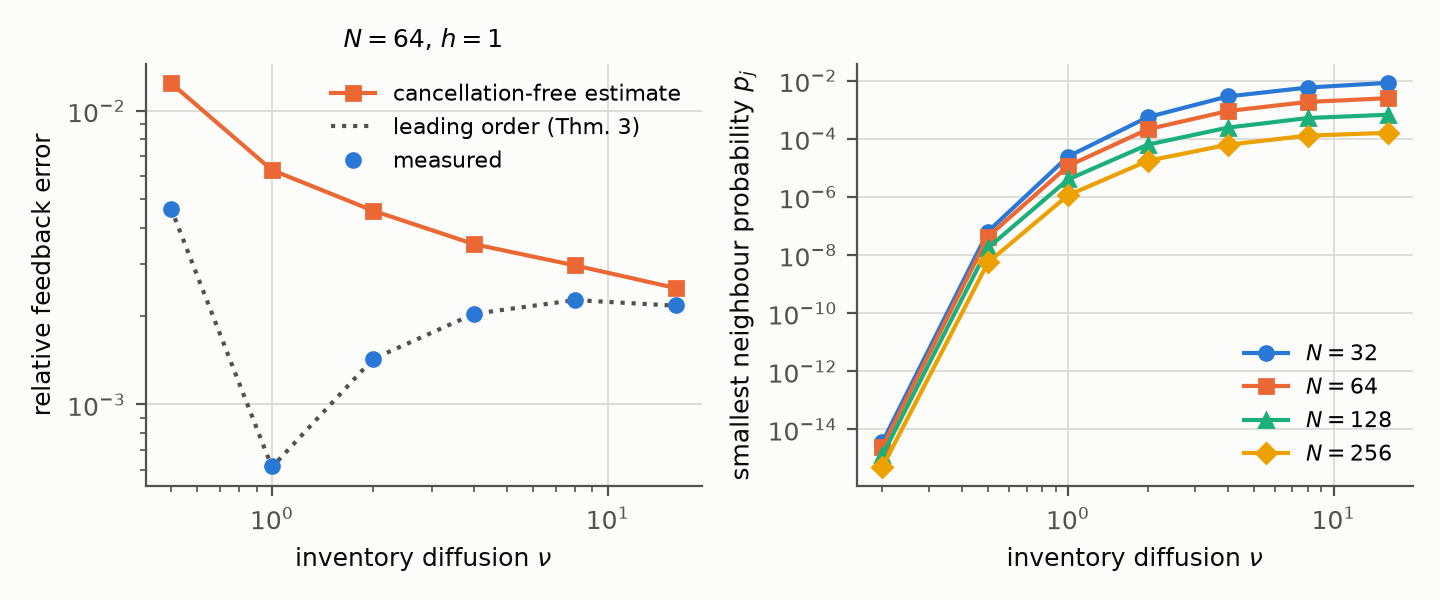
\includegraphics[width=0.96\textwidth]{step5_nu_tradeoff.png}
\caption{Left: measured grid error, the leading order of
Theorem~\ref{thm:grid} and the cancellation-free estimate. Right: smallest
normalised probability $p_j=\psi_j^2/\sum_k\psi_k^2$ among the four nodes
adjacent to $\X$.}
\label{fig:grid}
\end{figure}

\paragraph{Numerical validation.}
The semidiscrete system was integrated with a truncated-Taylor matrix
exponential \cite{almohy}. The half-width $L$ was fixed for each $\nu$ as the
smallest candidate whose rate differs by less than $10^{-5}$ from that on a
reference box, 1.6 times the largest candidate. Table~\ref{tab:grid} shows second-order convergence. Periodic and
Dirichlet boundaries differ by at most $\BoundaryDiff$ in the rate at $N=64$
for all seven values of $\nu$. Crank--Nicolson converges to the exponential
at second order in time. For $\lambda=0$ the grid agrees with the Riccati
rate to $\ZeroRiskErr$, and approaches the straight-line rate $\X/T$ as
$\Phi\to\infty$. Larger $\nu$ raises the probability of the nodes near $\X$
by twelve orders of magnitude between $\nu=0.2$ and $16$.

\begin{table}[!htbp]\centering\small\setlength{\tabcolsep}{4.5pt}
\begin{tabular}{@{}lccccc@{}}
\toprule
$\nu$ & $N=32$ & $N=64$ & $N=128$ & $N=256$ & $\min_jp_j$, $N=64$\\
\midrule
\TableG
\bottomrule
\end{tabular}
\caption{Measured relative rate error ($h=1$) and the smallest
neighbour probability. The low values near $\nu=1$ are the sign change of
Theorem~\ref{thm:grid}(iv).}
\label{tab:grid}
\end{table}

\section{Schr\"odingerisation}
\label{sec:schro}

\subsection{Shift picture and recovery window}

With an auxiliary coordinate $p$ and $w(0,p,\cdot)=g(p)\psi(0)$, the equation
$\partial_sw=\Hd\,\partial_pw$ becomes unitary after Fourier transform in
$p$, with generator $-\Hd\otimes D_\eta$ and norm
$\|\Hd\|\,\eta_{\max}$ \cite{jly}. On an eigenvector of $\Hd$ with
eigenvalue $E$ it is a shift, $w_E(s,p)=g(p+Es)\,\psi_E(0)$.

\begin{proposition}[shifted window]
\label{prop:window}
Let $g\in L^2(\mathbb R)$ with $g(p)=e^{-p}$ for $p\ge0$, and let $E_{\min}$
be the smallest eigenvalue of $\Hd$. For $s\ge0$,
$w(s,p)=e^{-p}\psi(s)$ for all $p\ge-E_{\min}s$. For $T>0$ and $\omega>0$, keeping outcomes
$p\in[-cT,-cT+\omega]$ with $c\le E_{\min}$ succeeds with probability
\begin{equation}
 \Psucc=\frac{e^{2cT}(1-e^{-2\omega})}{2\|g\|^2}\,
 \frac{\|\psi(T)\|^2}{\|\psi(0)\|^2}.
 \label{eq:psucc}
\end{equation}
\end{proposition}
\begin{proof}
For $p\ge-E_{\min}s$ every mode has $p+Es\ge0$, so
$g(p+Es)=e^{-p}e^{-Es}$. Integrate $e^{-2p}$ over the window.
\end{proof}

This is equivalent to subtracting a constant from $\Hd$, a freedom known in the
literature \cite{gujin}, and it needs no gates beyond relabelling $p$. We use
$c=0.98\,E_0$, with $E_0=\tfrac12\sum_i\sqrt{\lambda\mu_i}$ the continuum ground
level ($\mu_i$ the eigenvalues of $C$, $H=I$), and we verified $c\le E_{\min}$ on
every grid used by a costed configuration, at the benchmark and at all sweep
points. The points of the auxiliary grid are offset so that one of them is at
$p=-cT$; the circuit then prepares $g(p_l+o)$ for a known offset $o$, at no
extra cost. Without the offset the window starts at the next grid point and part
of the gain is lost. For the benchmark the shift raises $\Psucc$ by a factor
\WindowGain{} ($g_1$, $\eta_{\max}=20$).

\subsection{Discrete auxiliary grid}
\label{sec:wrap}

The circuit uses $N_p=2^{n_p}$ points on $[-L_p,L_p)$ with
frequencies $\eta_k=(k-\tfrac{N_p-1}2)\pi/L_p$, so that the shift is
performed by trigonometric interpolation. This choice makes the sign of each
bit of $k$ the sign of a block-encoding call (Eq.~\eqref{eq:segments}). For even $N_p$
the interpolant is antiperiodic over $2L_p$. The forward transform is
\[
 F_{kl}=N_p^{-1/2}e^{-i\eta_kp_l}=e^{i\pi(k-\frac{N_p-1}2)}N_p^{-1/2}
 e^{-2\pi ikl/N_p}e^{i\pi(N_p-1)l/N_p}.
\]
The phase in $k$ is a $Z$ gate up to a global phase, and the phase in $l$ is a product
of $n_p$ single-qubit rotations, which we charge. At the output it is diagonal in
$p$, commutes with the projector on the window and cancels in the Grover
iterate. The implemented transform agrees with the explicit matrix for
$N_p=4,8,16,32$. Two effects matter.

\emph{Wrap-around.} A mode with $ET$ comparable to $2L_p$ returns from the
other side. The spectrum of $\Hd$ extends to $\alpha_H=8\nu/\Delta x^2+V'\gg1$
(Section~\ref{sec:circuit}), and the initial data carry relative weight up to
$\WeightBench$ above $E=40$ on the $N=64$ grids of the benchmark. With $L_p=16$ or
32 and the smooth profiles below, the readout amplitudes at $N=64$ are wrong by
up to \UnsafeBench\% for the benchmark, and by more than their own size in
the sweep at $\lambda=4$. We choose
\begin{equation}
 L_p\ge\tfrac12\bigl(\alpha_HT+p_a+\omega+20\bigr),
 \label{eq:lp}
\end{equation}
with $p_a=-cT$ the window start and $\omega=3$. The cost is a few qubits: the
simulation time depends on $\eta_{\max}$ and not on $L_p$.

\begin{lemma}[wrap-around]
\label{lem:wrap}
Let $L>0$ and $|g(p)|\le e^{-|p|}$ for $|p|\ge R$. If $|y|\le2L-R$, then
\[
 \Bigl|\sum_{r\ne0}(-1)^rg(y+2Lr)\Bigr|\le\frac{2e^{-R}}{1-e^{-2L}} .
\]
\end{lemma}
\begin{proof}
For $r\ge1$ both $|y\pm2Lr|\ge R+2L(r-1)$. Sum the geometric series.
\end{proof}
The sum is the difference between $g$ and its antiperiodic extension, and
Eq.~\eqref{eq:lp} satisfies the hypothesis with $R=20$ for every $y=p+ET$ with $p$ in the
window and $0\le E\le\alpha_H$. A wrapped contribution therefore changes $w(T,p,\x)$ by at most
$2e^{-20}(1-e^{-2L_p})^{-1}\|\psi(0)\|$. The interpolant differs from the antiperiodic extension
by the aliasing error, which depends on the smoothness of $g$. Both are contained in the measured
amplitude errors below, which use the discrete transform.

\emph{Smoothness.} The kink of $g=e^{-|p|}$ limits convergence to first order
in $\Delta p$ \cite{jly}. As in the cut-off method of \cite{jlmpy} we
use a smooth $g$ that equals $e^{-p}$ on $p\ge0$. Ours blends into $e^{p}$ over
a width $w$,
\begin{equation}
 g_w(p)=S(p/w)\,e^{-p}+\bigl(1-S(p/w)\bigr)e^{p}\quad(-w<p<0),
 \label{eq:gw}
\end{equation}
with $S(y)=f(y+1)/[f(y+1)+f(-y)]$, $f(z)=e^{-1/z}$ for $z>0$ and 0
otherwise, and $g_w=e^{p}$ for $p\le-w$. Table~\ref{tab:profiles} and
Figure~\ref{fig:profiles} show the trade-off: a wider blend needs a smaller
$\eta_{\max}$ but lowers $\Psucc$.

\begin{table}[!htbp]\centering\small\setlength{\tabcolsep}{4.5pt}
\begin{tabular}{@{}lcccc@{}}
\toprule
$\eta_{\max}$ ($n_p$) & $e^{-|p|}$ & $g_{1/2}$ & $g_1$ & $g_2$\\
\midrule
\TableP
\bottomrule
\end{tabular}
\caption{Largest relative error of the readout amplitudes over all spans,
with $\Psucc$ in brackets ($\nu=2$, $N=64$, shifted window, exact
diagonalisation).}
\label{tab:profiles}
\end{table}

\begin{figure}[!htbp]\centering
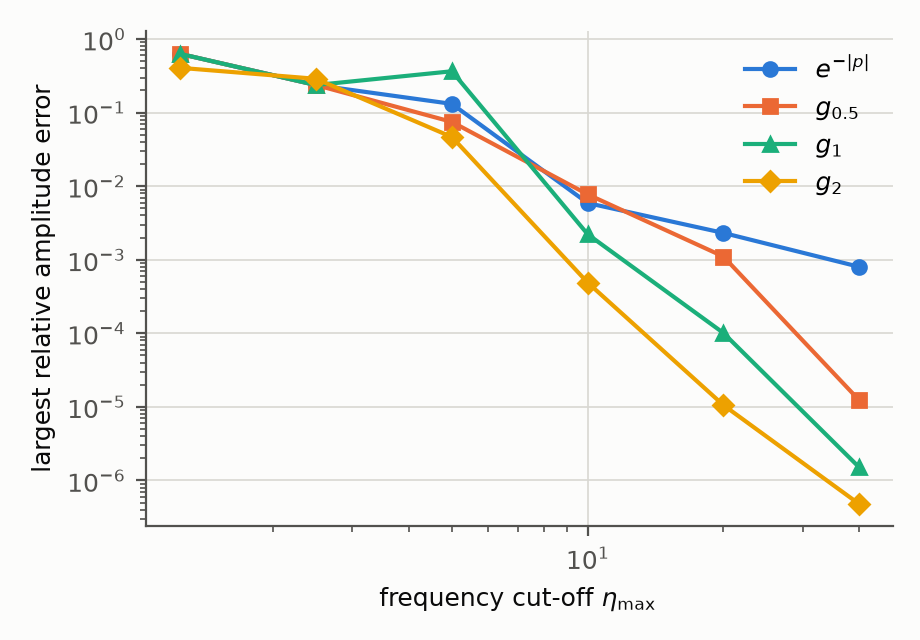
\includegraphics[width=0.50\textwidth]{step7_profiles.png}
\caption{Amplitude error of the recovered state against the frequency
cut-off for the four profiles of Table~\ref{tab:profiles}.}
\label{fig:profiles}
\end{figure}

\paragraph{Emulation at any grid size.}
For window points $p_l$, $w(T,p_l,\cdot)=f_l(\Hd)\psi(0)$ with $f_l$ band
limited. Its Chebyshev series on $[0,\alpha_H]$ converges once the degree
passes $\tfrac12\alpha_H\eta_{\max}T$, so the enlarged system can be
emulated without diagonalisation. This agrees with dense diagonalisation to
$4\times10^{-14}$ at $N=32$ and is used up to $N=256$ below.

\section{Circuit}
\label{sec:circuit}

\subsection{Block encoding}

For the two-asset case with $H=I$,
\begin{equation}
 \Hd-\alpha I=-\frac\nu{\Delta x^2}\sum_a\bigl(S_a+S_a^\dagger\bigr)-\tfrac12V'B
 +(V-V_m),\qquad
 \alpha=\frac{4\nu}{\Delta x^2}+\frac{V'}2,
 \label{eq:lcu}
\end{equation}
where $S_a$ is a cyclic increment and $B$ a comparator, taken in the mean of
Lemma~\ref{lem:comp}. Let $q(\x)$ be the top $m$ bits of
$5\x^\top C\x/\Delta x^2=5z_1^2+5z_2^2+10\rho\,z_1z_2$, with $z_a=x_a/\Delta x$
and $10\rho$ an integer, scaled by $2^k>\max 5\x^\top C\x/\Delta x^2$.
The strict inequality keeps $q$ representable in $m$ bits.

\begin{lemma}[comparator potential]
\label{lem:comp}
Let $B=\sum_r|r\rangle\langle r|\otimes(-1)^{[r<q(\x)]}$ on an $m$-qubit register.
Then $\langle+^m|B|+^m\rangle=\operatorname{diag}(1-2q/2^m)$. Hence
$\tfrac12V'(I-B)$ encodes $V_m=V'q/2^m$ with
$V'=\tfrac{\lambda\Delta x^2}{4\nu}\tfrac{2^k}5$ and
$0\le V-V_m<V'2^{-m}$.
\end{lemma}
\begin{proof}
$2^{-m}\sum_r(-1)^{[r<q]}=1-2q/2^m$, and $q$ is a truncation.
\end{proof}

\begin{lemma}[effect of rounding]
\label{lem:round}
If $0\le V-V_m\le\delta$ entrywise and the initial data are nonnegative, then
$\psi\le\psi_m\le e^{T\delta}\psi$ entrywise.
\end{lemma}
\begin{proof}
$-\Hd$ has nonnegative off-diagonal entries, so $e^{-s\Hd}$ preserves
positivity and is monotone decreasing in the diagonal potential. Compare
with the potentials $V$ and $V-\delta$.
\end{proof}

The circuit encodes $\Hd-\alpha I$ with normalisation $\alpha$. The spectrum of $\Hd$
lies in $[0,\alpha_H]$ with $\alpha_H=2\alpha$, so encoding $\Hd$ itself would double the
walk length. The removed constant contributes $e^{i\eta\alpha T}$, a translation in $p$: its
integer part relabels the window and its fractional part is added to the offset $o$ of the prepared
profile. The four shifts have equal weight, so PREPARE is one $R_y$ rotation
(kinetic against potential) and Hadamards. SELECT applies $-S_a^{\pm1}$ as
controlled increments and flips the direction bit, which makes it Hermitian.
The potential branch squares and multiplies the coordinates, forms
$5z_1^2+5z_2^2+10\rho z_1z_2$ by shifts and additions, compares the top $m$
bits with $r$, applies a phase and uncomputes.

\paragraph{Verification.} For $n=2$ and $m=2$, built as an explicit
512-dimensional unitary, we verified $\mathrm{SELECT}^2=I$, that the encoded block
equals $(\Hd-\alpha I)/\alpha$ with $V$ replaced by $V_m$, the bound of
Lemma~\ref{lem:comp}, and that the walk operator has eigenphases
$\pm\arccos[(E-\alpha)/\alpha]$ for every eigenvalue $E$. At the costed sizes we
compiled SELECT to $X$, CNOT, AND, $Z$ and $CZ$ gates with measurement-based uncomputation
\cite{gidney}. It is a permutation of basis states with signs, so the gate list can be simulated
exactly on basis states. For all \CompileCount{} selected configurations (benchmark and sweeps,
both readouts) it acts correctly on every grid point and on $2\times10^5$ random basis
states, and returns all work qubits to zero. We charge the AND count and the workspace of this circuit. As a
cross-check, Qualtran's block costs \cite{qualtran} for the same layout differ from it by between $-\CompileMax\%$ and
$+\CompileMin\%$; the largest shortfall of the block costs is at $\rho=0$, where their in-place squarer is cheaper than
the one that we could verify.

\subsection{Evolution}

In offset binary, $\eta=\sum_{j<n_p}s_j2^{j-1}\Delta\eta$ with $s_j=\pm1$, so
\begin{equation}
 e^{i\eta\Hd T}=\prod_{j<n_p}e^{is_j\tau_j\Hd},\qquad
 \tau_j=2^{j-1}\Delta\eta\,T,\qquad\sum_j\tau_j=\eta_{\max}T .
 \label{eq:segments}
\end{equation}
The sign $s_j$ multiplies the block encoding and costs a Clifford $Z$ per
SELECT. Each factor is a generalised quantum signal processing (GQSP)
polynomial \cite{gqsp} in the qubitised walk \cite{qubitization}. Following
\cite{berry} we charge $K_j+3$ walk steps per segment ($K_j+1$ directionally controlled, two
controlled), where $K_j\ge\alpha\tau_j$ is even. Standard quantum signal processing needs about
$2K_j$. Let $\theta_j=2\sum_{k>K_j}|J_k(\alpha\tau_j)|$ be the Jacobi--Anger tail. The truncated
polynomial pair is rescaled below norm one and completed to a unitary \cite{berry}. The
completion cancels in the $|+\rangle\to|+\rangle$ block of the signal qubit, which then differs from
$e^{is_j\tau_j\Hd}$ by at most $2\theta_j$, but it leaks amplitude up to $2\sqrt{\theta_j}$ to
$|-\rangle$, and the next segments can return part of it. Over $n_p$ segments of equal tail
$\theta$ the success branch errs by at most $2n_p\theta+2n_p^2\theta$ to leading order, so we require
$\theta_j\le\eps_{\rm coh}/[4n_p(n_p+1)]$, where $\eps_{\rm coh}$ is the error allowed for the
state of one run; the other half of $\eps_{\rm coh}$ is for rotations.

\subsection{Gate and qubit accounting}
\label{sec:account}

Toffoli and logical-AND gates count as 4 T \cite{gidney}; uncomputing an AND
by measurement is free. SELECT is charged at the AND count of its compiled circuit, in which the arithmetic is computed and
uncomputed; multi-controlled phases use Qualtran 0.7 \cite{qualtran}. Rotations cost
$3\log_2(1/\epsilon)+2$ T \cite{rs} (leading term plus a small allowance),
four per walk step. Two reflections per step account for directional control.
The initial Gaussian and $g$ are prepared by QROM-driven Grover--Rudolph
\cite{gr,babbush}, with about $2^{2n+1}+2n\,b_{\rm rot}$ and
$2^{n_p+1}+n_p\,b_{\rm rot}$ Toffolis, where $b_{\rm rot}$ is the rotation
precision in bits. The two quantum Fourier transforms
are charged $n_p^2$ Toffolis each. Preparation is \PrepShareA\% of a run at
1\% (readout A).

Qubits are counted at the peak of the potential oracle: $2n$ position,
$n_p$ auxiliary, $3+m$ PREPARE, one signal qubit, the workspace of the compiled SELECT, and $b_{\rm rot}$
phase-gradient qubits. Coordinates have $n+3$ bits for readout A and $n+1$ for readout B.

\section{Readout}
\label{sec:readout}

\subsection{A: pointwise amplitude estimation}

Let $b_j^2$ be the probability of finding $p$ in the window and $\x=\x_j$, so
$b_j=\sqrt{\Psucc p_j}$. Relative errors $\delta_j$ of the four amplitudes
change the rate by
\[
 |\Delta v_a|\le\frac\nu d\bigl[-\log(1-\delta_{a+})
 -\log(1-\delta_{a-})\bigr],\qquad 0\le\delta_{a\pm}<1.
\]
A target $\eps$ with grid error $\eps_{\rm grid}$ gives the finite budget
\begin{equation}
 L=(\eps-\eps_{\rm grid})\,\|\vv^*\|\,\frac{d}{2\sqrt2\,\nu},
 \qquad \delta=1-e^{-L},
 \label{eq:budget}
\end{equation}
of which 70\% goes to amplitude estimation and 10\% each to
Schr\"odingerisation, coherent simulation (GQSP truncation and rotation
synthesis) and potential rounding (through Lemma~\ref{lem:round}). We require
$\eps_{\rm grid}\le\eps/2$, with the charged error of Section~\ref{sec:grid}.
If the three deterministic errors total at most $0.3\delta$ relative to the
reference amplitude and the estimation error is at most $0.7\delta$ relative
to the prepared amplitude, their product lies in
$[1-\delta,1/(1-\delta)]$, and each log error is at most $L$. The calculation is
conditional on the allocated errors. The Schr\"odingerisation error of a profile at
some $\eta_{\max}$ is replaced by its maximum over the larger tested $\eta_{\max}$, so
that a dip is not used. For grids larger than $64^2$ the selection uses the profile
error at $64^2$; the selected benchmark and sweep configurations are then checked at
their actual grids, rounded potentials and auxiliary grids (Section~\ref{sec:emu}).

Amplitude estimation \cite{bhmt} with $M_j=2^{t_j}$ phase outcomes has relative
error at most $\pi/(M_jb_j)+\pi^2/(2M_j^2b_j^2)$ with probability at least
$8/\pi^2$. The standard phase-estimation circuit uses $M_j-1$ Grover
iterations; we charge $2M_j+1$ coherent runs, including state
preparation and its inverse. With a semiclassical Fourier
transform \cite{griffiths} it needs one extra qubit. The exponents $t_j$ are
chosen per node to meet its allocated error. The median of 11 repetitions gives
at least 95\% joint confidence for the four estimates (binomial bound).
Iterative variants \cite{iqae} may be cheaper.

\subsection{B: sampling the feedback matrix}

In the quadratic model the recovered state is a Gaussian with
$|\psi(\x,T)|^2\propto e^{-\x^\top P_T\x/(4\nu)}$, that is covariance
$\Sigma=2\nu P_T^{-1}$. Measuring $p$ and $\x$ and keeping the accepted
samples gives
\begin{equation}
 \hat P=2\nu\hat\Sigma^{-1},\qquad \hat\vv(\x)=\tfrac12\hat P\x
 \quad\text{for every }\x .
 \label{eq:sampling}
\end{equation}
The mean is zero by symmetry. Neither $\nu$ nor $\X$ matters
(Lemma~\ref{lem:scale}), so no node need coincide with $\X$. The error
metric is $\|(\hat P-P_T)P_T^{-1}\|_2$, which is uniform in $\x$. Its
systematic part $r$ adds the grid error and the Schr\"odingerisation plus
rounding error in norm, so they cannot cancel; both are measured against the
known $P_T$, and we require $r\le\eps/2$. A coherent error $e$ of the state changes the second-moment
matrix by at most $8\mathsf L^2e/\sqrt{\Psucc}$ to first order, where $\mathsf L$ is the half-width of the box; we
allow for $0.01\eps$ in the metric and charge $0.02\eps$. For $n_s$ accepted
samples the 96\% quantile of the statistical part is $\kappa/\sqrt{n_s}$ with
$\kappa=\KappaB$ (large-sample Wishart limit, simulated), so
$n_s=[\kappa/(0.98\eps-r)]^2$. The number of runs is the smallest for which at
least $n_s$ samples are accepted with probability 0.99 (exact binomial). The
product of the two probabilities exceeds 0.95; the first is asymptotic in $n_s$ and is
tested by the emulation.

This readout needs no amplitude amplification, but it uses the Gaussian form
of $\psi$. It does not extend to non-quadratic problems.

\section{Results}
\label{sec:results}

\subsection{Resource counts}

\begin{table}[!htbp]\centering\footnotesize\setlength{\tabcolsep}{4pt}
\begin{tabular}{@{}lccc@{}}
\toprule
target $\eps$ & 5\% & 1\% & 0.1\%\\
\midrule
\TableA
\bottomrule
\end{tabular}
\caption{Readout A (amplitude estimation): best configuration found, with charged grid error at most $\eps/2$, for
$\nu\in\{1,2,4,8,16\}$, $N\in\{32,64,128,256\}$, $h\in\{1,2,4,8,16\}$ and
the profiles of Table~\ref{tab:profiles} (the three cheapest admissible auxiliary grids are costed for each).}
\label{tab:a}
\end{table}

\begin{table}[!htbp]\centering\small\setlength{\tabcolsep}{4.5pt}
\begin{tabular}{@{}lccc@{}}
\toprule
target $\eps$ & 5\% & 1\% & 0.1\%\\
\midrule
\TableB
\bottomrule
\end{tabular}
\caption{Readout B (sampling): best configuration found for 95\% confidence on the
error of the whole feedback matrix.}
\label{tab:b}
\end{table}

\begin{table}[!htbp]\centering\small\setlength{\tabcolsep}{4.5pt}
\begin{tabular}{@{}lcccccccc@{}}
\toprule
& $\x$ & $p$ & PREPARE & signal & arithmetic & phase grad. & QAE control & total\\
\midrule
\TableQ
\bottomrule
\end{tabular}
\caption{Logical qubits by register.}
\label{tab:q}
\end{table}

\begin{figure}[!htbp]\centering
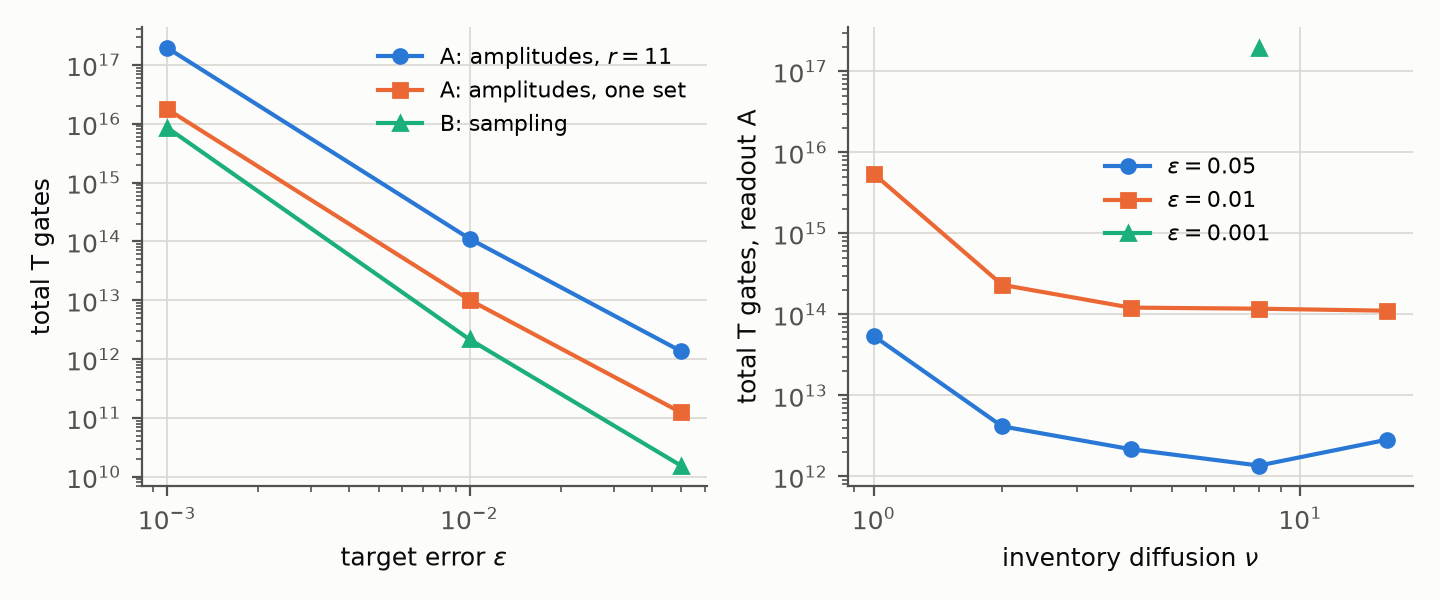
\includegraphics[width=0.96\textwidth]{tcount.png}
\caption{Left: T count against target error for readout A (one estimate set,
and the median of 11) and readout B. Right: readout A against $\nu$; the cost
falls steeply from $\nu=1$ and is nearly flat for $\nu\gtrsim4$. At 0.1\% only $\nu=8$ has an admissible configuration in the search.}
\label{fig:t}
\end{figure}

Tables~\ref{tab:a}--\ref{tab:q} give the best configurations found. At 1\%, readout A needs
\QAOne{} qubits and $\TAOne$ T gates. Readout B needs \QBOne{} qubits and $\TBOne$ T gates and returns
the full feedback matrix. The ratio of \RatioAB{} between them compares unlike
guarantees: A repeats a worst-case bound 11 times, B uses the actual distribution of its
estimator. A single set of amplitude estimates ($\TAsingleOne$ T gates) is \RatioABSingle{} times
the cost of B and succeeds in \SingleMin--\SingleMax\% of the emulated trials (Table~\ref{tab:e}). The
gap narrows at 0.1\%, where sampling costs $1/\eps^2$ runs against $1/\eps$
for amplitude estimation (Figure~\ref{fig:t}). Three factors dominate.
\begin{enumerate}
\item \emph{Runs.} One estimate set of readout A uses $\ReadoutRuns$ runs and
readout B $\RunsBOne$ runs.
\item \emph{Walk steps}, about $\alpha\,\eta_{\max}T$ per run: \StepsA{} for A and \StepsB{} for B.
\item \emph{The potential oracle}, \OracleMin--\OracleMax\% of a walk step.
\end{enumerate}
At one T gate per microsecond executed serially, readout A at 1\% would take
\SerialYearsA{} years and readout B \SerialDaysB{} days, without
error-correction overhead.

\subsection{What the auxiliary variable costs}
\label{sec:direct}

$\Hd$ is Hermitian and nonnegative, so the auxiliary variable is not necessary.
The walk encodes $x=\Hd/\alpha-1\in[-1,1]$, and with $\beta=\alpha T$
\begin{equation}
 e^{-T\Hd}=e^{-\beta(1+x)}=e^{-\beta}\Bigl[I_0(\beta)+2\sum_{k\ge1}(-1)^kI_k(\beta)T_k(x)\Bigr],
 \label{eq:direct}
\end{equation}
which may be truncated at $K\approx\sqrt{2\beta\log(2/\mathrm{tol})}$ \cite{sachdeva}. Let
$\tau_K=2e^{-\beta}\sum_{k>K}I_k(\beta)$ be the uniform Bessel-tail bound. The truncated
polynomial has norm at most $1+\tau_K$ on the spectrum. For the GQSP resource estimate we scale it by
$1/(1+\tau_K)$ to obtain a contraction; the resulting approximation error is at most $2\tau_K$.
The resource script chooses $\tau_K\leq\varepsilon_{\rm state}/4$, so this error is at
most $\varepsilon_{\rm state}/2$. A degree-$K$ Chebyshev polynomial is a Laurent polynomial
of degree $K$ in the walk, and GQSP implements the shifted degree-$2K$ polynomial with
$2K$ controlled walk steps. This quadratic saving for Hermitian semigroups is known
\cite{gslw,jmz}. Table~\ref{tab:direct} costs it on the grids and budgets of
Tables~\ref{tab:a} and~\ref{tab:b}, with the same arithmetic. The state succeeds with the
norm ratio of Lemma~\ref{lem:scale} instead of the shifted $\Psucc$, the Fourier transforms and the
$p$ register disappear, and the share of the Schr\"odingerisation error goes to the polynomial. At 1\% the
saving is a factor \DirA{} in T gates for A and \DirB{} for B, and \DirQA{} and \DirQB{} qubits.
Schr\"odingerisation is the more general method: it applies to non-Hermitian generators,
which arise when the inventory has a drift. For the present class of
problems it should be read as an upper bound that the direct polynomial improves.
The GQSP phases and complement polynomial have not been compiled, so these T counts are analytic estimates.
The finite-grid check in \nolinkurl{simulation/direct_polynomial.py} applies the contraction-scaled series to the tested input vectors;
it checks those instances but does not prove a uniform bound or verify a circuit. Readout probabilities and run counts use the
scaled polynomial output.

\begin{table}[!htbp]\centering\small\setlength{\tabcolsep}{4.5pt}
\begin{tabular}{@{}lcccccc@{}}
\toprule
& walk steps & (Schr.) & runs & (Schr.) & T gates (ratio) & qubits\\
\midrule
\TableX
\bottomrule
\end{tabular}
\caption{The direct polynomial \eqref{eq:direct} on the grids of Tables~\ref{tab:a} and~\ref{tab:b}; in brackets the
corresponding entries with Schr\"odingerisation and the ratio of T counts. For A, runs are per estimate set
and T gates for the median of 11.}
\label{tab:direct}
\end{table}

\subsection{Emulation}
\label{sec:emu}

Both pipelines were emulated with the costed parameters. The emulation
includes the rounded potential and the discrete auxiliary grid, but not the
GQSP truncation and gate-synthesis errors
(which are only budgeted). For readout A the amplitude estimates are drawn
from the canonical amplitude-estimation outcome law using all $M$ distinct
outcomes and floating-point probabilities; for readout B we
draw the costed number of runs, reject with probability $1-\Psucc$, and fit
Eq.~\eqref{eq:sampling}. Each experiment has 2000 trials.

\begin{table}[!htbp]\centering\footnotesize\setlength{\tabcolsep}{4pt}
\begin{tabular}{@{}lcccccccc@{}}
\toprule
& \multicolumn{6}{c}{readout A} & \multicolumn{2}{c}{readout B}\\
\cmidrule(lr){2-7}\cmidrule(l){8-9}
$\eps$ & amp.\ error (budget) & exact-amp. & 95\% quant. & $r{=}11$ & $r{=}3$ & $r{=}1$ & uniform & at $\X$\\
\midrule
\TableE
\bottomrule
\end{tabular}
\caption{Emulation. ``Amp.\ error'' is the relative error of the recovered
amplitudes against their budget; ``exact-amp.'' is the rate error with
exact amplitudes; the remaining columns of A are the 95\% quantile for $r=11$
and the percentage of trials within $\eps$ for medians of $r$ estimates. For B
the percentage within $\eps$ uses the uniform metric and the error at $\X$.}
\label{tab:e}
\end{table}

\begin{figure}[!htbp]\centering
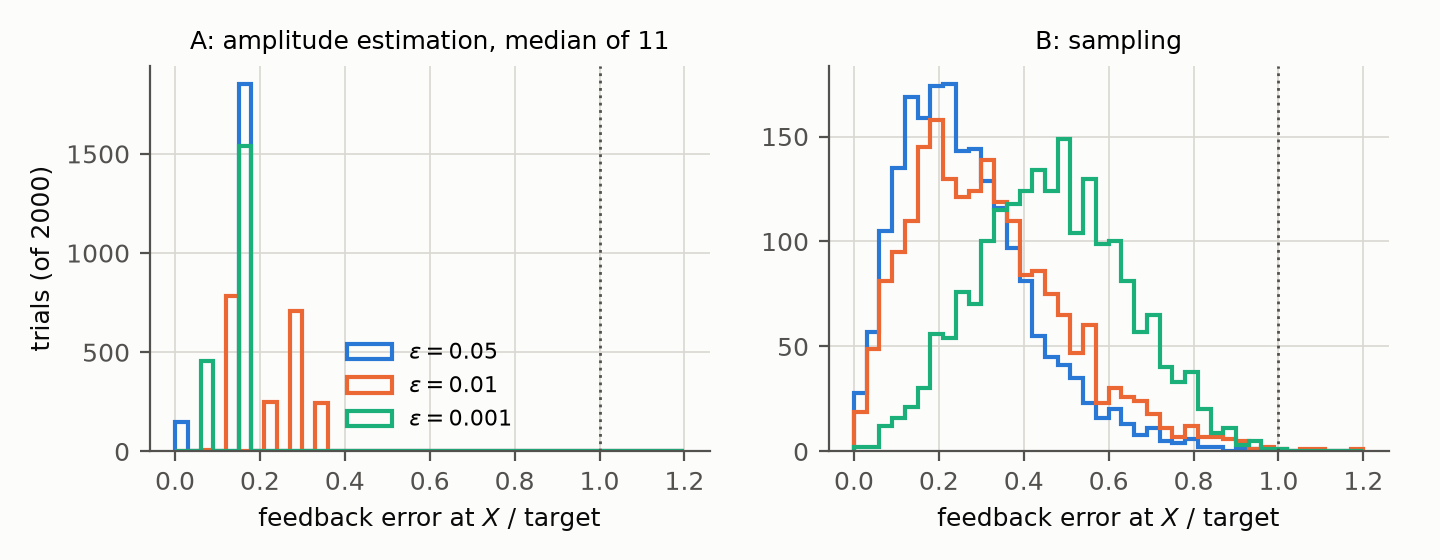
\includegraphics[width=0.96\textwidth]{step10_emulation.png}
\caption{Distribution of the emulated rate error at $\X$ relative to the
target (2000 trials each); the dotted line is the target.}
\label{fig:e}
\end{figure}

In every run of Table~\ref{tab:e} and Figure~\ref{fig:e} the measured amplitude error is
inside its budget. For A with $r=11$ and for B the one-sided 99.9\% Clopper--Pearson lower bound
on the success probability is at least \LowerBound\%. This supports the 95\% target
for the emulated pipelines; it is not a bound that covers GQSP truncation and synthesis errors. Readout A
with $r=3$ succeeds in at least \ThreeMin\% of trials, which would divide its T count by $11/3$; this is an
observation about these instances. The narrow histograms of A reflect the
quantised outcomes of amplitude estimation with large $M_j$.

We also separate potential rounding from Schr\"odingerisation at the four
nodes, with both differences relative to the unrounded semigroup amplitude.
Across the three benchmark targets and six 1\% sweep points, their largest
measured errors are respectively 0.667 and 0.965 of their individual allocations.
The latter occurs at the 5\% benchmark. For that $32^2$ case, dense
eigendecomposition and the Chebyshev recovery agree in relative amplitude to
$2.9\times10^{-15}$. These floating-point comparisons are not enclosures and
do not emulate GQSP or gate synthesis.

\subsection{Sensitivity to parameters}

Table~\ref{tab:s} repeats the 1\% search for other correlations and risk
aversions. Readout A varies between $\SweepAmin$ and $\SweepAmax$ T gates,
readout B between $\SweepBmin$ and $\SweepBmax$. Larger $\lambda$ increases
both, through the potential and the smaller recovery probability. In the
emulations of all rows the target is met in at least \SweepWithinA\% (A) and \SweepWithin\% (B)
of 2000 trials. Some optima lie at the largest $\nu$ of the search, where the
count is flat in $\nu$ (Figure~\ref{fig:t}).

\begin{table}[!htbp]\centering\small\setlength{\tabcolsep}{4.5pt}
\begin{tabular}{@{}lccccccc@{}}
\toprule
& \multicolumn{3}{c}{readout A} & \multicolumn{4}{c}{readout B}\\
\cmidrule(lr){2-4}\cmidrule(l){5-8}
$\rho$; $\lambda$ & T gates & qubits & $\nu$; grid & T gates & qubits & $\Psucc$ & within $\eps$ (\%)\\
\midrule
\TableS
\bottomrule
\end{tabular}
\caption{Best 1\% configurations found for different correlations and risk aversions. The row
$0.4;1$ is the benchmark.}
\label{tab:s}
\end{table}

\subsection{Scaling with the number of assets}
\label{sec:scaling}

For $M$ assets the continuum formulas give a resource model
without simulation. We take $H=I$, $C=(1-\rho)I+\rho\mathbf 1\mathbf 1^\top$,
$\rho=0.4$, $\Phi=1.5I$, $\X=(3,1,3,1,\dots)$, spacing $0.25\sqrt\nu$ and
$\eps=1\%$, and count coherent runs. Readout A is minimised over $\nu$ and
$d$; the sampling row is $\kappa_M^2/(\tfrac12\eps)^2/\Psucc$ with $\kappa_M$ from a
Wishart simulation. Lemma~\ref{lem:scale} supplies the norm ratio. Table~\ref{tab:m}
also gives $\Psucc$ for the exact shift $c=E_0$.

\begin{table}[!htbp]\centering\small\setlength{\tabcolsep}{4.5pt}
\begin{tabular}{@{}ccccccc@{}}
\toprule
$M$ & $\Psucc$, $p\ge0$ & $c=0.98E_0$ & $c=E_0$ & runs A & runs B ($p\ge0$) & runs B (shifted)\\
\midrule
\TableM
\bottomrule
\end{tabular}
\caption{Continuum model of the success probability and of the number of coherent runs at $\eps=1\%$.
Extrapolation for $M>2$; one set of amplitude estimates for A; runs use $c=0.98E_0$ unless $p\ge0$ is stated.}
\label{tab:m}
\end{table}

Readout A's coherent-run count grows by about \GrowthA{} per added asset over the range
$M=4$ to $10$. The point probability falls with the grid-cell volume, and amplitude
estimation uses a number of calls proportional to the inverse point amplitude. The success probability is a product over the
eigenmodes of $C$. Each mode with eigenvalue $\mu$ contributes
$\|e^{-(\hat H_\mu-c_\mu)T}\psi_\mu(0)\|^2/\|\psi_\mu(0)\|^2$, with $\hat H_\mu$ its one-dimensional operator and
$c_\mu$ its share of $c$. For $c_\mu$ at the mode's ground level this is at most one, with equality only if
the initial data are the ground state. Here $M-1$ modes have $\mu=1-\rho$. Each such repeated mode
contributes a factor \FacPlain{} without a shift, \FacMargin{} for $c=0.98E_0$ and
\FacExact{} for $c=E_0$. These are repeated-mode factors, not the total finite-$M$ ratios,
because the remaining common-mode eigenvalue changes with $M$. The shift moves the repeated-mode
factor from \FacPlain{} close to one; it does not remove the exponential contribution. Together with the growth of $\kappa_M^2$, which is linear in $M$, the runs of
readout B increase by a factor \GrowthBTotal{} between $M=1$ and $10$. The classical Riccati
solution is polynomial in $M$, so for quadratic models sampling does not beat it.

\section{Non-quadratic data}
\label{sec:nonquad}

All configurations of Tables~\ref{tab:a} and~\ref{tab:s} use $\nu\ge4$, where $\X$ lies near the
centre of the state. Proposition~\ref{prop:feedback} allows this because the quadratic feedback does not
depend on $\nu$. We now ask what the same circuit costs when it does.

\subsection{The amplitude barrier}

\begin{proposition}[amplitude barrier]
\label{prop:barrier}
Let $\psi_i=e^{-W_i/(4\nu)}$ on a finite grid and $p_j=\psi_j^2/\sum_i\psi_i^2$. For all $j,k$,
\begin{equation}
 p_j\le\exp\Bigl[-\frac{W_j-W_k}{2\nu}\Bigr].
 \label{eq:barrier}
\end{equation}
If moreover $W_j-W_k\ge w\ge0$ and the recovered control has a relative bias of at least $\beta\nu$ ($\beta>0$) that
must not exceed $\eps$, then $p_j\le e^{-w\beta/(2\eps)}$.
\end{proposition}
\begin{proof}
Keep the term $k$ of the sum. The second part uses $\nu\le\eps/\beta$.
\end{proof}

The readout amplitude is thus at most $\sqrt{\Psucc}\,e^{-(W_j-\min W)/4\nu}$. Estimating an amplitude $b$ to
relative precision $\delta$ takes $\Theta(1/(\delta b))$ uses of the state preparation
\cite{bhmt,nayakwu}, so the runs of readout A grow like $e^{(W_j-\min W)/4\nu}$. For
smooth solutions the viscous control has an asymptotic series in $\nu$ \cite{flemingsouganidis}, and its bias is
proportional to $\nu$ unless the first correction has zero gradient, as it has for quadratic
data. A target $\eps$ then requires $\nu=O(\eps)$, and direct pointwise readout costs $e^{\Theta(1/\eps)}$.
In the normalisation of \cite{jinliu}, Eq.~\eqref{eq:barrier} reads
$q=|\langle x|u\rangle|^2\le e^{-(S(x)-\min S)/\nu}$. The proof of their Lemma 12
derives the factor
$J=(1/q+1/\|\mathbf u\|^2)^2/\|\mathbf u\|^2$ in the cost expression; the lemma statement
omits it. For a unit-norm initial state and contractive evolution, $\|\mathbf u\|^2\leq1$,
so $J\geq q^{-2}$. Their choice $\nu=O(\eps_{\min}^2/d^2)$ concerns an absolute
Hamilton--Jacobi value error and dimension $d$, not this paper's relative control error.

\subsection{Recentring on a classical extremal}

\begin{proposition}[recentring]
\label{prop:recentre}
Let $H\succ0$, $V:\mathbb R^M\to\mathbb R$, and let $G:\mathbb R^M\to\mathbb R^M$ be any vector field. Let
\begin{equation}
 \boldsymbol\xi'=-2\nu H^{-1}\boldsymbol\alpha,\qquad\boldsymbol\alpha'=-G(\boldsymbol\xi),\qquad
 \gamma'=\nu\,\boldsymbol\alpha\!\cdot\!H^{-1}\boldsymbol\alpha+G(\boldsymbol\xi)\!\cdot\!\boldsymbol\xi-V(\boldsymbol\xi),
 \label{eq:char}
\end{equation}
and let $\phi(\mathbf y,s)$, differentiable and $C^2$ in $\mathbf y$, satisfy
\begin{equation}
 \phi_s=\nu\nabla\!\cdot(H^{-1}\nabla\phi)-\bigl[V(\boldsymbol\xi+\mathbf y)-V(\boldsymbol\xi)-G(\boldsymbol\xi)\!\cdot\!\mathbf y\bigr]\phi .
 \label{eq:phi}
\end{equation}
Then $\psi(\x,s)=e^{\boldsymbol\alpha\cdot\x+\gamma}\,\phi(\x-\boldsymbol\xi,s)$ satisfies
$\psi_s=\nu\nabla\!\cdot(H^{-1}\nabla\psi)-V\psi$, and where $\phi>0$
\begin{equation}
 -2\nu H^{-1}\nabla\log\psi(\x,s)=-2\nu H^{-1}\boldsymbol\alpha-2\nu H^{-1}\nabla\log\phi(\x-\boldsymbol\xi,s).
 \label{eq:refcontrol}
\end{equation}
\end{proposition}
\begin{proof}
With $E=e^{\boldsymbol\alpha\cdot\x+\gamma}$, $\psi_s=E[(\boldsymbol\alpha'\!\cdot\x+\gamma')\phi-\boldsymbol\xi'\!\cdot\nabla\phi+\phi_s]$ and
$\nabla\!\cdot(H^{-1}\nabla\psi)=E[\nabla\!\cdot(H^{-1}\nabla\phi)+2\boldsymbol\alpha\!\cdot H^{-1}\nabla\phi+\boldsymbol\alpha\!\cdot H^{-1}\boldsymbol\alpha\,\phi]$.
Insert Eqs.~\eqref{eq:char} and~\eqref{eq:phi}: the gradient terms cancel and the remaining
coefficient of $\phi$ is $-V(\x)$.
\end{proof}

Take $V=\ell/(4\nu)$ for a running cost $\ell$, $G=\nabla V$ and
$\boldsymbol\pi=-4\nu\boldsymbol\alpha$. Equation~\eqref{eq:char} becomes
$\boldsymbol\xi'=\tfrac12H^{-1}\boldsymbol\pi$, $\boldsymbol\pi'=\nabla\ell(\boldsymbol\xi)$, the extremals of
Eq.~\eqref{eq:cost} in time remaining, and the first term of Eq.~\eqref{eq:refcontrol} is the control
$\tfrac12H^{-1}\boldsymbol\pi$ of the extremal. The quantum computer estimates only the
correction to it. Three properties matter for the cost.
\begin{enumerate}
\item The generator of Eq.~\eqref{eq:phi} is Hermitian. For convex $\ell$ its potential is nonnegative. For quadratic $\ell$
it is $V(\mathbf y)$, so that operator, circuit and $E_{\min}$ are unchanged and only the prepared state differs:
$\phi(\mathbf y,0)\propto\exp\{-[g(\boldsymbol\xi_0+\mathbf y)-\boldsymbol\pi_0\!\cdot\!\mathbf y]/(4\nu)\}$ for a terminal cost $g$.
For other $\ell$ the potential depends on $s$, and the simulation must be time dependent.
\item Let the extremal end at $\boldsymbol\xi(T)=\X$, and put $\widetilde W=-4\nu\log\phi$. By Eq.~\eqref{eq:refcontrol}
$\nabla\widetilde W(0,T)$ is twice $H$ times the correction. If the extremal is optimal
and $W$ is convex, then $\widetilde W$ has its minimum at $0$ up to the viscous bias, and the exponent of
Eq.~\eqref{eq:barrier} no longer grows as $\nu\to0$.
\item The reference may be inexact. If the minimum of $\widetilde W$ is at distance $\eta$ from $0$, the exponent is
$O(\eta^2/\nu)$: a reference accurate to $O(\sqrt\nu)$ suffices, while the answer is wanted to $O(\nu)$.
\end{enumerate}

\subsection{A quartic terminal penalty}

We keep the benchmark and replace the terminal cost by
$g(\mathbf y)=\tfrac12\mathbf y^\top\Phi\mathbf y+\kappa\sum_ay_a^4$. The operator is that of the
benchmark. Since its kernel is Gaussian, the viscous rate is a two-dimensional integral over the terminal
point and the inviscid rate a Newton solve, so both references are available to machine precision.
For $\kappa=0$ the bias vanishes to $\NqBiasZero$ at every $\nu$, as
Proposition~\ref{prop:feedback} states. For $\kappa=0.1$ it is $\NqSlope\,\nu$ for small $\nu$ (relative,
Figure~\ref{fig:nq} left), and $W_0(\X,T)=\NqW$. The reference of the recentred readout is the extremal of the
quadratic model ($\kappa=0$) through $\X$; its control is wrong by \NqRef\% for
$\kappa=0.1$ and \NqRefHard\% for $\kappa=0.5$.

Table~\ref{tab:nq} compares three readouts. \emph{Direct}: Eq.~\eqref{eq:readout} at the cheapest $\nu$ and span, using
continuum stencil values and a finite-difference estimate of the norm ratio. \emph{Extrapolated}: the same at $\nu$, $2\nu$ and $4\nu$ with Richardson weights.
\emph{Recentred}: a grid simulation, costed with the circuit of Section~\ref{sec:circuit}. Its bias, span error
and grid error are measured against the exact references and added in norm, with the largest grid error over
all tested spans, and must stay below $\eps/2$; the Schr\"odingerisation and rounding errors are measured on the
costed configuration, and the readout is emulated. The direct and extrapolated run counts use the asymptotic
$2\pi/(\delta b)$ query estimate; the recentred count uses the implemented power-of-two QAE schedule.
Only recentred T gates are costed, including the median of 11. The norm-ratio estimate for direct and
extrapolated uses a $128^2$ finite-difference solve; doubling the grid to $256^2$ changes $P_{\rm succ}$ by
0.040--0.063\% over the selected viscosities. This is a convergence check, not an error enclosure.
At $\kappa=0.1$ and 1\% the direct readout needs
$\nu\approx\NqNuOne$ and $\NqDirectOne$ runs, extrapolation reduces this to $\NqRichOne$, and recentring to
$\NqRecOne$, with \NqQOne{} qubits and $\NqTOne$ T gates in total. At 0.1\% the direct readout is out of reach and the recentred one
needs $\NqTTenth$ T gates. The recentred counts are smaller than those of the benchmark because
the reference supplies most of the answer; they are the cost of a correction. All emulated success probabilities have a
99.9\% lower bound of at least \NqLower\%.

For $\kappa=0.5$ at 0.1\% neither the direct readout nor the recentred one with the quadratic reference has an
admissible configuration in our search ($\nu\ge5\times10^{-4}$): the bias requires a $\nu$ for which the reference is too far
from the optimum. A better reference, for instance one Newton step on the terminal condition, would be needed.

\begin{table}[!htbp]\centering\footnotesize\setlength{\tabcolsep}{3.2pt}
\begin{tabular}{@{}lccccccccc@{}}
\toprule
& \multicolumn{3}{c}{direct} & extrap. & \multicolumn{5}{c}{recentred}\\
\cmidrule(lr){2-4}\cmidrule(lr){5-5}\cmidrule(l){6-10}
$\kappa$; $\eps$ & $\nu$ & $\min b_j$ & runs & runs & $\nu$ & grid; $h$ & runs & T gates & qubits\\
\midrule
\TableN
\bottomrule
\end{tabular}
\caption{Quartic terminal penalty. Runs are coherent runs per set of four amplitude estimates; T gates
include the median of 11. Extrapolation uses three values of $\nu$.}
\label{tab:nq}
\end{table}

\begin{figure}[!htbp]\centering
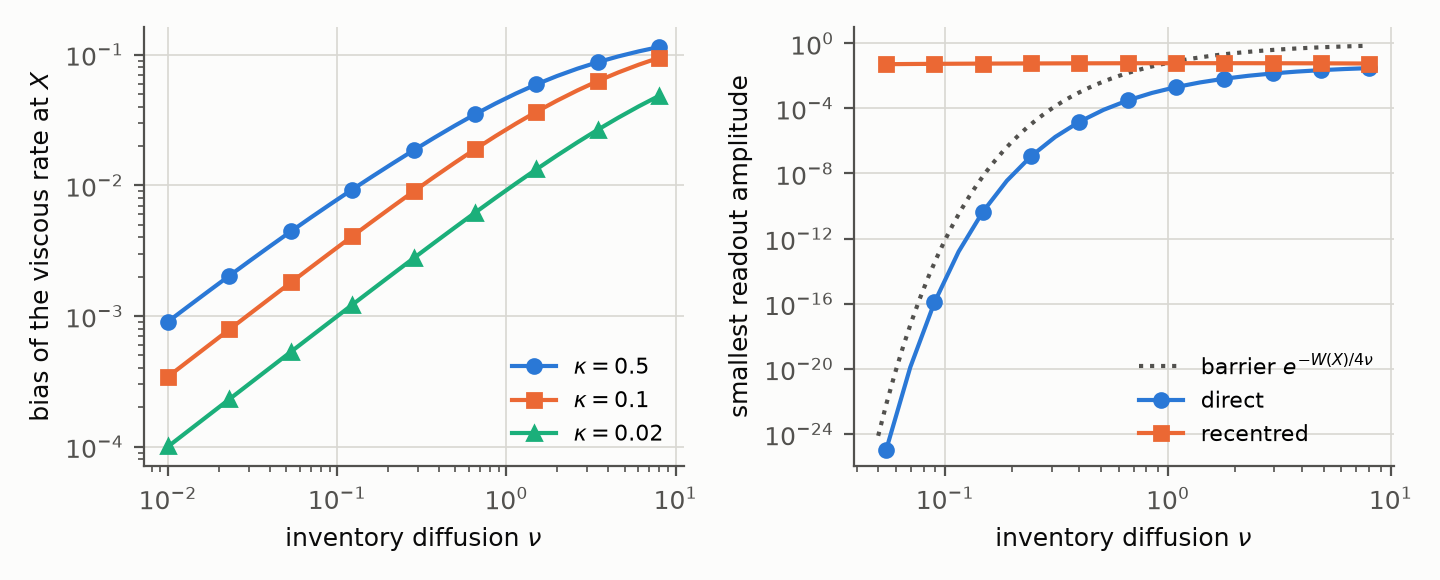
\includegraphics[width=0.96\textwidth]{nonquadratic.png}
\caption{Left: relative bias of the viscous rate at $\X$. Right: smallest readout amplitude for $\kappa=0.1$ at
spacing $0.25\sqrt\nu$ and span $0.5\sqrt\nu$, with and without recentring; the dotted line is the factor of
Eq.~\eqref{eq:barrier}.}
\label{fig:nq}
\end{figure}

\section{Discussion}
\label{sec:discussion}

\paragraph{What the estimate says.} Solving the two-asset benchmark at 1\%
takes \QBOne--\QAOne{} logical qubits and $\TBOne$--$\TAOne$ T gates with
Schr\"odingerisation, and \DirB{} to \DirA{} times fewer T gates with a direct polynomial. The counts
are dominated by repetition: an estimate set uses $\ReadoutRuns$ runs for A,
and sampling uses $\RunsBOne$ runs for B. Improvements that reduce the number
of runs (iterative amplitude estimation, cheaper confidence boosting,
variance reduction for sampling) are worth more than compressing a
single run.

\paragraph{Role of the benchmark.} A quadratic model was chosen so that
every stage has a checkable answer. Section~\ref{sec:nonquad} shows that it is
also an unrepresentative one: the freedom to take $\nu$ large is a property of
quadratic data, and resource estimates for Cole--Hopf methods made on such data, or that
leave the point probability inside an unspecified constant, do not extend to other data.
Recentring restores a moderate cost if a classical reference of moderate accuracy is available.

\paragraph{Classical competitors.} A grid method with pointwise readout should not be compared only with classical
grids. For the deterministic problem \eqref{eq:cost} with convex costs, the control at one point is found by trajectory
optimisation, whose cost is polynomial in $M$. At fixed $\nu$ the Feynman--Kac formula gives the same
pointwise value by Monte Carlo without a grid, and the recentring of
Proposition~\ref{prop:recentre} is then importance sampling \cite{kappenruiz}. The amplitude
of a grid point, in contrast, falls with the grid volume (Section~\ref{sec:scaling}), recentred or not. A
credible advantage needs a problem that these methods do not solve and an observable that is cheaper
than the control at a point.

\paragraph{Limitations.}
\begin{itemize}
\item Counts are logical. Error correction, layout, routing, magic-state
distillation and measurement latency are not included.
\item Configurations are selected with the help of the known solution: through the reference values in the error estimates of
readout A, and through the measured error for readout B and for the recentred readout. An
application would need a-priori bounds.
\item Theorem~\ref{thm:grid} covers $H=I$ and central differences on a
uniform lattice. The constants of the numerical grid-error estimate are sampled
floating-point values, charged at twice their sampled value, not validated
enclosures. Readout-A counts that use this estimate are conditional on the
sampled maxima upper-bounding the true spatial and temporal extrema.
\item The circuit is specialised to $H=I$ and integer $10\rho$. General
impact matrices and correlations need weighted LCU terms and constant
multiplications.
\item Only SELECT is compiled to gates. GQSP phases, rotation synthesis, QROM and Fourier transforms are
charged with standard formulas, and their errors are budgeted but not emulated. The QAE cost uses the
canonical scheme with a median of 11.
\item The $M$-asset table is a continuum model for the number of runs. It does
not include the cost per run and has not been simulated for $M>2$.
\item Recentring is costed for quadratic running costs only.
\item The parameters are synthetic, and the model omits spread costs,
participation limits and sales-only constraints.
\end{itemize}

\section{Conclusion}

We costed, and emulated end to end, a route from a multi-asset execution
HJB to its optimal rate: compatible-diffusion Cole--Hopf, a grid with a
proved error expansion, Schr\"odingerisation with a smooth profile
and a shifted window, a qubitised evolution, and two readouts. For a
two-asset benchmark at 1\% it needs \QBOne--\QAOne{} logical qubits and between
$\TBOne$ and $\TAOne$ T gates; classical Riccati integration is faster by
many orders of magnitude. The exercise separates three effects that asymptotic statements hide. Grid errors of the control
cancel at isolated parameter values, and a resource count tuned on a known answer inherits the cancellation. The low cost of
pointwise readout is a property of quadratic data; where the feedback has a bias linear in $\nu$, direct readout is exponential in
the inverse accuracy. A change of variables along a classical extremal removes that factor, and for quadratic running costs it does
not change the circuit.

\appendix
\section{Proof of Theorem~\ref{thm:grid}}
\label{app:proof}

% Shared by Paper.tex and ../WorkPlan.tex.
\paragraph{Riccati matrix.}
For $H=I$, $Y'=\tfrac12Z$ and $Z'=2\lambda CY$. Equation~\eqref{eq:form} gives
$(Y\mathbf w)\cdot(Z\mathbf w)\ge\mathbf w^\top\Phi\mathbf w$. With $\mathbf w=Y^{-1}\x$ this is
$\x^\top P_s\x\ge\mathbf w^\top\Phi\mathbf w$, and $Y$ is bounded on $[0,T]$, so $P_s\succeq mI$
for some $m>0$ and all $s\in[0,T]$. $P_s$ is symmetric because
$(Y\mathbf w)\cdot(Z\mathbf w')-(Y\mathbf w')\cdot(Z\mathbf w)$ is constant and vanishes at $0$.

\paragraph{Maximum principle.}
\emph{Let $u$ be bounded on the lattice times $[0,T]$, $u(\cdot,0)\le0$, and
$u'\le\nu\sum_aD_{2,a}u-Vu+g(s)$ with $V\ge0$, $g\ge0$. Then $u(\cdot,s)\le G(s)=\int_0^sg$.}
Put $\xi(\x)=1+|\x-\X|^2$, so that $\nu\sum_aD_{2,a}\xi=2\nu M=:c$, and
$w=u-G-\epsilon\bigl(\xi+(c+1)s\bigr)$ with $\epsilon>0$. Since $u$ is bounded and $\xi$ has
finite sublevel sets, $w$ has a maximum, at $(\x_1,s_1)$ say. Suppose it is positive. Then
$s_1>0$, so $w'\ge0$ there, $\sum_aD_{2,a}w\le0$ and $u>0$. But
\[
 w'\le\nu\sum_aD_{2,a}u-Vu-\epsilon(c+1)=\nu\sum_aD_{2,a}w+\epsilon c-Vu-\epsilon(c+1)<0 ,
\]
a contradiction. Let $\epsilon\to0$. The argument uses only nonnegative jump rates and a
barrier, so it also covers boxes. If
$|u'-\nu\sum_aD_{2,a}u+Vu|\le g$ and $u(\cdot,0)=0$, the statement for $\pm u$ gives $|u|\le G$; in particular bounded solutions are unique.

\paragraph{Existence.}
With $\kappa=2M\nu/\Delta^2$, solutions are the fixed points of
\[
 u(\x,s)\mapsto e^{-(V+\kappa)s}u(\x,0)
 +\int_0^se^{-(V+\kappa)(s-r)}\frac\nu{\Delta^2}\sum_{a,\pm}u(\x\pm\Delta\mathbf e_a,r)\,dr,
\]
a contraction on bounded continuous functions in the norm $\sup e^{-\mu s}|u|$ for large $\mu$,
because $V\ge0$.

\paragraph{(i) Consistency and stability.}
Taylor's theorem with the Lagrange remainder gives, for $L\in C^{2J+4}$,
\[
 \Bigl|\frac{L(\Delta)+L(-\Delta)-2L(0)}{\Delta^2}-\sum_{j=0}^Jc_j\Delta^{2j}L^{(2j+2)}(0)\Bigr|
 \le c_{J+1}\Delta^{2J+2}\sup|L^{(2J+4)}| .
\]
Let $S_K=\sum_{k\le K}\Delta^{2k}\psi_k$ and apply this to $\psi_k$ with $J=K-k$. Reordering the
sums in Eq.~\eqref{eq:hier},
\[
 \partial_sS_K=\nu\sum_aD_{2,a}S_K-VS_K+r,\qquad
 |r|\le\Delta^{2K+2}\,\nu\sum_{k\le K}c_{K-k+1}\sum_a\bigl\|\partial_a^{2(K-k)+4}\psi_k(s)\bigr\|_\infty .
\]
The maximum principle for $\psi_\Delta-S_K$, which vanishes at $s=0$, is
Eq.~\eqref{eq:bk}, provided the $\psi_k$ exist and the norms are finite.

\paragraph{(i) Existence of the hierarchy.}
For a polynomial $q$, $\partial_a(q\psi)=(\mathcal D_aq)\psi$ with
$\mathcal D_aq=\partial_aq+\varphi_aq$, and $\partial_s\psi=\nu\nabla^2\psi-V\psi$. Hence
Eq.~\eqref{eq:hier} for $\psi_k=p_k\psi$ is
\[
 \partial_sp_k=\nu\nabla^2p_k-\tfrac12(P_s\x)\!\cdot\!\nabla p_k
 +\nu\sum_{i<k}c_{k-i}\sum_a\mathcal D_a^{2(k-i)+2}p_i,\qquad p_k(\cdot,0)=0 .
\]
The operator maps polynomials of degree at most $n$ to such polynomials, and the source is a
known polynomial. This is a linear ordinary differential equation with continuous
coefficients in a finite-dimensional space, so $p_k$ exists on $[0,T]$. Every
$\partial_a^n\psi_k$ is a polynomial, with coefficients continuous in $s$, times
$\psi\le e^{-m|\x|^2/(8\nu)}/\sqrt{\det Y}$. It is bounded, and its supremum norm is continuous in $s$.

\paragraph{(ii)} For $k=1$ the source is
$\tfrac\nu{12}\sum_a\mathcal D_a^41$ and
$\mathcal D_a^41=\varphi_a^4+6\varphi_a^2\varphi_{aa}+3\varphi_{aa}^2$. Let $A$, $B$, $D$ solve, with zero
initial data,
\begin{equation}
\begin{aligned}
 A_s&=-\tfrac12(P_s\x)\!\cdot\!\nabla A+\tfrac1{3072}\sum_a(P_s\x)_a^4,\\
 B_s&=-\tfrac12(P_s\x)\!\cdot\!\nabla B+\nabla^2A-\tfrac1{128}\sum_a(P_s)_{aa}(P_s\x)_a^2,\\
 D_s&=\nabla^2B+\tfrac1{64}\sum_a(P_s)_{aa}^2 .
\end{aligned}
\label{eq:abd}
\end{equation}
Then $\nu^{-3}A+\nu^{-2}B+\nu^{-1}D$ solves Eq.~\eqref{eq:chi}, whose solution is unique.

\paragraph{(iii)}
On the segments $\X+t\mathbf e_a$, $|t|\le d_0$, the Gaussian $\psi(\cdot,T)$ is bounded below by a
positive constant. Part (i) with $K=2$ gives
$\psi_\Delta/\psi=1+\Delta^2p_1+\Delta^4p_2+O(\Delta^6)$, so for small $\Delta$, uniformly in $|t|\le d_0$,
\[
 \log\psi_\Delta=\log\psi+\Delta^2p_1+\Delta^4q+O(\Delta^6),\qquad q=p_2-\tfrac12p_1^2 .
\]
Insert this in Eq.~\eqref{eq:readout}. The first term gives $v_a^*$ exactly, the second $\Delta v_a$. The polynomial $q$ is Lipschitz on the
segment, so the third contributes $O(\Delta^4)$ after division by $2d$. The last contributes
$O(\Delta^6)/d=O(\Delta^5)$ since $d\ge\Delta$.

\paragraph{(iv)}
Fix $\mathbf w\ne0$ and let $\x(s)=Y_s\mathbf w$, $\mathbf z(s)=Z_s\mathbf w=P_s\x(s)$, so $\dot\x=\tfrac12P_s\x$. Along this
curve Eq.~\eqref{eq:abd} integrates to
$A=\tfrac1{3072}\int_0^s\sum_az_a^4\,dr>0$, because $\x\cdot\mathbf z\ge\mathbf w^\top\Phi\mathbf w>0$ implies
$\mathbf z\ne0$. Let $h=\nabla^2A$ at $\x(s)$ and $\mathbf p_a=P_s\mathbf e_a$. Differentiating the equation
for $A$ twice,
\[
 h'=-\tfrac12(hP_s+P_sh)+\tfrac1{256}\sum_az_a^2\,\mathbf p_a\mathbf p_a^\top,\qquad
 (Y^\top hY)'=\tfrac1{256}\sum_az_a^2\,(Y^\top\mathbf p_a)(Y^\top\mathbf p_a)^\top\succeq0 ,
\]
so $h\succeq0$. Since $P_s'=2\lambda C-\tfrac12P_s^2$, $(P_s^{-1})'=\tfrac12I-2\lambda P_s^{-1}CP_s^{-1}$ and
\[
 \bigl[\tr(hP_s^{-1})\bigr]'=-\tfrac12\tr h+\tfrac1{256}\sum_az_a^2(P_s)_{aa}
 -2\lambda\tr(hP_s^{-1}CP_s^{-1}).
\]
Add twice this to $B'=\tr h-\tfrac1{128}\sum_az_a^2(P_s)_{aa}$: the first two terms cancel and
Eq.~\eqref{eq:mono} remains. Its right-hand side is $\le0$ because $h\succeq0$ and
$P_s^{-1}CP_s^{-1}\succeq0$. Both terms in the bracket vanish at $s=0$, so
$B\le-2\tr(hP_s^{-1})$. Finally $\x^\top h\x=12A>0$ by homogeneity, so $h\ne0$, and
$h\succeq0$, $P_s^{-1}\succ0$ give $\tr(hP_s^{-1})>0$. Every point is of the form $Y_s\mathbf w$, which
proves Eq.~\eqref{eq:signs}. The last statement is Euler's identity,
$\x\cdot\nabla A=4A$ and $\x\cdot\nabla B=2B$.\hfill\qedsymbol


\section{Machine-checked proofs}
\label{app:lean}

The folder \nolinkurl{lean/} contains a Lean~4 development on Mathlib (both v4.36.0).
It proves the formal statements listed in Table~\ref{tab:lean} without
\lean{sorry} and without \lean{native_decide}. These are counterparts of the
paper's statements, with the qualifications below. A script collects the axioms of all its
declarations and fails if any lies outside Lean's standard three
(\lean{propext}, \lean{Classical.choice}, \lean{Quot.sound}).

\begin{table}[!htbp]\centering\footnotesize\setlength{\tabcolsep}{4pt}
\begin{tabular}{@{}ll>{\raggedright\arraybackslash}p{6.1cm}@{}}
\toprule
statement & module & theorem\\
\midrule
Proposition~\ref{prop:feedback} & \lean{GeneralImpact} & \lean{proposition_one}\\
Lemma~\ref{lem:scale} & \lean{Feedback}, \lean{GeneralImpact} & \lean{scale_invariance}, \lean{norm_ratio}\\
Riccati facts & \lean{Riccati} & \lean{exists_riccatiFlow}, \lean{P_symm}, \lean{P_deriv}, \lean{exists_coercive}\\
maximum principle & \lean{MaxPrinciple} & \lean{maximum_principle}, \lean{abs_le_of_residual}\\
Taylor bound & \lean{SecondDifference} & \lean{second_difference_bound}\\
Theorem~\ref{thm:grid}, existence and (i) & \lean{GridTheorem} & \lean{grid_theorem_main}\\
\quad explicit $B_K$ & \lean{GridExpansion} & \lean{grid_expansion}\\
\quad hierarchy & \lean{Hierarchy}, \lean{PolyGauss} & \lean{exists_hierarchy}\\
Theorem~\ref{thm:grid}(ii) & \lean{Leading}, \lean{Radial} & \lean{eval_source_one}, \lean{p_one_eq}, \lean{A_homog}, \lean{B_homog}\\
Theorem~\ref{thm:grid}(iii) & \lean{Leading} & \lean{rate_expansion}\\
Theorem~\ref{thm:grid}(iv) & \lean{SignTheorem}, \lean{Radial} & \lean{A_pos}, \lean{B_le}, \lean{B_neg}, \lean{radial_error_sign}\\
$\psi$ prefactor, $\theta=\tfrac12\log\det Y$ & \lean{GeneralImpact} & \lean{logDet_deriv}, \lean{theta_eq}\\
Proposition~\ref{prop:box} & \lean{Truncation} & \lean{box_truncation}\\
Proposition~\ref{prop:window} & \lean{Window} & \lean{shifted_window}, \lean{window_weight}\\
Lemma~\ref{lem:wrap} & \lean{Wrap} & \lean{wrap_bound}\\
Lemma~\ref{lem:comp} & \lean{Comparator} & \lean{comparator_potential}, \lean{comparator_truncation}\\
Lemma~\ref{lem:round} & \lean{Rounding} & \lean{rounding}\\
Proposition~\ref{prop:barrier} & \lean{Barrier} & \lean{amplitude_barrier}, \lean{barrier_of_bias}\\
Proposition~\ref{prop:recentre} & \lean{Recentre} & \lean{recentre}, \lean{recentred_feedback}\\
\bottomrule
\end{tabular}
\caption{Formal counterparts in the folder \texttt{lean/ExecutionProofs/}; see the qualifications below.}
\label{tab:lean}
\end{table}

Not formalised: the numbers (numerical values of $B_K$, $U$ and the error-bound estimates, and
all resource counts), Eq.~\eqref{eq:cert}, the circuit constructions with their error analysis (including the GQSP leakage
bound), the error analysis of the readouts, and results quoted from the literature. In
\lean{shifted_window} the mode decomposition is an assumption, and \lean{window_weight} is the window integral; the normalisation of
Eq.~\eqref{eq:psucc} is one further division. \lean{norm_ratio} is stated for arbitrary $P\succ0$ and $\det Y$, and
$P_T\succ0$ is formalised for $H=I$. \lean{grid_theorem_main} states (i) with some
constant for each fixed truncation order; \lean{grid_expansion} gives the
corresponding bound for any supplied primitive of the norm bounds. The
formal statement \lean{proposition_one} constructs a Gaussian solution and
its feedback, but does not state the block-matrix exponential formula or the
optimal-control verification theorem. The paper's presentation of one
infinite hierarchy and its explicit integral constant also goes beyond the
quantifiers of \lean{grid_theorem_main} alone. \lean{wrap_bound} concerns the images of $g$ and not the interpolant.
\lean{barrier_of_bias} takes the bias inequality as a hypothesis; for the quartic example the bias is measured.
\lean{recentre} takes the derivatives in Eqs.~\eqref{eq:char} and~\eqref{eq:phi} as hypotheses.

\section{Verification of the reference model}
\label{app:verify}

Scripts in \nolinkurl{simulation/} assert the following.
\begin{itemize}
\item \emph{Symbolic.} The two-asset HJB, its feedback, the Riccati
reduction and the sign map from Eq.~16 of \cite{bdg} (with $R=0$) are
rederived with SymPy.
\item \emph{Hard-liquidation case.} With $\x(T)=0$ and the benchmark
parameters, $J^*=13.8105120319$ and $\vv(0)=(4.0488,1.6640)$. Direct
quadrature reproduces $J^*$ to $3\times10^{-15}$. The sales-only condition
$X_1/X_2\le15.989$ is satisfied by $3$, and the minimum rates
$2.5063$, $0.6931$ occur at $t=1$.
\item \emph{Discrete trajectory problem.} The block-tridiagonal minimiser
has inventory error $6.9\times10^{-5}$, $4.4\times10^{-6}$,
$2.7\times10^{-7}$, $1.7\times10^{-8}$ for 16, 64, 256, 1024 steps.
\item \emph{Finite-penalty Riccati.} The block exponential
\eqref{eq:riccati} agrees with fourth-order Runge--Kutta integration, with
maximum entry errors $1.0\times10^{-10}$, $6.4\times10^{-12}$ and
$3\times10^{-15}$ for 128, 256 and 4096 steps.
An independent adaptive integration over 60 random cases in dimensions
$1,2,4$, including non-identity positive-definite $H$, differs from the block
exponential by at most $3.0\times10^{-12}$ in relative Frobenius norm. This
is a numerical check, not a proof for all inputs. A separate check of
Eq.~\eqref{eq:verification} with 20 random two-asset instances and sinusoidal
controls has maximum absolute residual $3.5\times10^{-10}$.
\end{itemize}

\section{Reproducibility}
\label{app:code}

The ancillary file named \texttt{research-sources.zip} contains the
simulation scripts, saved results and Lean sources. Every table entry and
headline count is generated from the result files by
\nolinkurl{simulation/make_numbers.py}. A few constants in the running text, and
Appendix~\ref{app:verify}, are quoted by hand from the same files and from
the scripts' assertions. The scripts use NumPy, SciPy, SymPy, Matplotlib and
Qualtran (versions in \nolinkurl{simulation/requirements.txt}). \nolinkurl{simulation/run_all.sh} runs the
whole pipeline in order in about two hours on 16 cores; \nolinkurl{make_numbers.py} and \nolinkurl{figures.py} then write the
tables and figures. The proofs are checked from \nolinkurl{lean/} with \texttt{lake exe cache get}, \texttt{lake build} and
\texttt{lake env lean scripts/AxiomCheck.lean}.

\paragraph{Use of AI tools.} Generative AI systems (Anthropic Claude and OpenAI Codex) were used to write code, Lean proofs and text, and to
cross-review the manuscript. The author is responsible for the content.

\begin{thebibliography}{99}\small
\bibitem{ac} R.~Almgren and N.~Chriss, Optimal execution of portfolio transactions, \emph{J.~Risk} 3(2), 5--39 (2001).
\bibitem{bdg} P.~Bergault, F.~Drissi and O.~Gu\'eant, Multi-asset optimal execution and statistical arbitrage strategies under Ornstein--Uhlenbeck dynamics, \emph{SIAM J.~Financial Math.}~13(1), 353--390 (2022), arXiv:2103.13773.
\bibitem{jlyshort} S.~Jin, N.~Liu and Y.~Yu, Quantum simulation of partial differential equations via Schr\"odingerisation, \emph{Phys.~Rev.~Lett.}~133, 230602 (2024), arXiv:2212.13969.
\bibitem{jly} S.~Jin, N.~Liu and Y.~Yu, Quantum simulation of partial differential equations: Applications and detailed analysis, \emph{Phys.~Rev.~A} 108, 032603 (2023); preprint titled Quantum simulation of partial differential equations via Schr\"odingerisation: technical details, arXiv:2212.14703.
\bibitem{jlm} S.~Jin, N.~Liu and C.~Ma, Schr\"odingerisation based computationally stable algorithms for ill-posed problems in partial differential equations, arXiv:2403.19123.
\bibitem{jlmpy} S.~Jin, N.~Liu, C.~Ma, Y.~Peng and Y.~Yu, On the Schr\"odingerization method for linear non-unitary dynamics with optimal dependence on matrix queries, arXiv:2505.00370.
\bibitem{gujin} A.~Gu and S.~Jin, Quantum simulation of a class of highly-oscillatory transport equations via Schr\"odingerisation, arXiv:2501.10176.
\bibitem{nguyentura} H.~A.~Nguyen and A.~Tura, Quantum simulation of dissipative acoustic and elastic waves by Schr\"odingerization: absorbing boundaries and explicit polynomial-size circuits, arXiv:2611.02357.
\bibitem{hjlz} J.~Hu, S.~Jin, N.~Liu and L.~Zhang, Quantum circuits for partial differential equations via Schr\"odingerisation, \emph{Quantum} 8, 1563 (2024), arXiv:2403.10032.
\bibitem{wang2026conservation} K.~Wang, J.~Hu and L.~Zhang, An efficient explicit implementation of a quantum algorithm with quantum advantage for nonlinear scalar conservation laws, arXiv:2608.09675 (2026).
\bibitem{jlybc} S.~Jin, N.~Liu and Y.~Yu, Quantum circuits for the heat equation with physical boundary conditions via Schr\"odingerisation, arXiv:2407.15895.
\bibitem{lchs} D.~An, J.-P.~Liu and L.~Lin, Linear combination of Hamiltonian simulation for nonunitary dynamics with optimal state preparation cost, \emph{Phys.~Rev.~Lett.}~131, 150603 (2023), arXiv:2303.01029.
\bibitem{jmz} S.~Jin, C.~Ma and E.~Zuazua, Transmutation based quantum simulation for non-unitary dynamics, arXiv:2601.03616.
\bibitem{gslw} A.~Gily\'en, Y.~Su, G.~H.~Low and N.~Wiebe, Quantum singular value transformation and beyond: exponential improvements for quantum matrix arithmetics, \emph{Proc.~51st ACM STOC}, 193--204 (2019), arXiv:1806.01838.
\bibitem{sachdeva} S.~Sachdeva and N.~K.~Vishnoi, Faster algorithms via approximation theory, \emph{Found.~Trends Theor.~Comput.~Sci.}~9(2), 125--210 (2014).
\bibitem{jinliu} S.~Jin and N.~Liu, Quantum algorithms for viscosity solutions to nonlinear Hamilton--Jacobi equations based on an entropy penalisation method, arXiv:2512.07919.
\bibitem{jlywass} S.~Jin, N.~Liu and Y.~Yu, Schr\"odingerization based quantum algorithms for regularized Wasserstein proximal operators, arXiv:2606.28752.
\bibitem{uchida} F.~Uchida, K.~Miyamoto, S.~Yamazaki, K.~Fujisawa and N.~Yoshida, Quantum simulation of Burgers turbulence: nonlinear transformation and direct evaluation of statistical quantities, arXiv:2412.17206.
\bibitem{sasaki} S.~Sasaki, K.~Endo and M.~Muramatsu, Hamiltonian simulation for nonlinear partial differential equation by Schr\"odingerization, \emph{Sci.~Rep.}~16, 11743 (2026), arXiv:2508.01640.
\bibitem{krovi} H.~Krovi, Quantum algorithms to simulate quadratic classical Hamiltonians and optimal control, arXiv:2404.07303.
\bibitem{wangriccati} J.~Wang, Y.~Wang, B.~Li, J.-P.~Liu and Z.~Ji, Near-optimal quantum algorithm and complexity analysis for Riccati problems, arXiv:2609.37207.
\bibitem{huanglqr} X.~Huang, C.~\'Alvarez~Yuste, N.~Guseynov, N.~Liu and J.~Gonz\'alez-Conde, Quantum algorithms for optimal control: large-scale finite-horizon linear-quadratic regulation, arXiv:2610.26843.
\bibitem{rosenberg} G.~Rosenberg, P.~Haghnegahdar, P.~Goddard, P.~Carr, K.~Wu and M.~L\'opez~de~Prado, Solving the optimal trading trajectory problem using a quantum annealer, \emph{IEEE J.~Sel.~Top.~Signal Process.}~10(6) (2016), arXiv:1508.06182.
\bibitem{chakrabarti} S.~Chakrabarti \emph{et al.}, A threshold for quantum advantage in derivative pricing, \emph{Quantum} 5, 463 (2021), arXiv:2012.03819.
\bibitem{stamatopoulos} N.~Stamatopoulos and W.~J.~Zeng, Derivative pricing using quantum signal processing, \emph{Quantum} 8, 1322 (2024), arXiv:2307.14310.
\bibitem{guseynov} N.~Guseynov, N.~Liu, C.~S.~Pun and T.~Vaidya, End-to-end PDE-based quantum algorithms for multi-asset option pricing under local and stochastic volatility, arXiv:2605.26610.
\bibitem{jennings} D.~Jennings, M.~Lostaglio, R.~B.~Lowrie, S.~Pallister and A.~T.~Sornborger, The cost of solving linear differential equations on a quantum computer: fast-forwarding to explicit resource counts, \emph{Quantum} 8, 1553 (2024), arXiv:2309.07881.
\bibitem{pocrnic} M.~Pocrnic, P.~D.~Johnson, A.~Katabarwa and N.~Wiebe, Constant-factor improvements in quantum algorithms for linear differential equations, arXiv:2506.20760.
\bibitem{penuel} J.~Penuel \emph{et al.}, Detailed assessment of calculating drag force with quantum computers: explicit time-evolution precludes exponential advantage for nonlinear differential equations, arXiv:2406.06323.
\bibitem{gyongykrylov} I.~Gy\"ongy and N.~Krylov, Accelerated finite difference schemes for second order degenerate elliptic and parabolic problems in the whole space, \emph{Math.~Comp.}~80, 1431--1458 (2011), arXiv:0905.3299.
\bibitem{gurevich} P.~Gurevich, Asymptotics of parabolic Green's functions on lattices, arXiv:1504.02673.
\bibitem{kappen} H.~J.~Kappen, Linear theory for control of nonlinear stochastic systems, \emph{Phys.~Rev.~Lett.}~95, 200201 (2005), arXiv:physics/0411119.
\bibitem{todorov} E.~Todorov, Efficient computation of optimal actions, \emph{Proc.~Natl.~Acad.~Sci.}~106, 11478--11483 (2009).
\bibitem{hopf} E.~Hopf, The partial differential equation $u_t+uu_x=\mu u_{xx}$, \emph{Comm.~Pure Appl.~Math.}~3, 201--230 (1950).
\bibitem{cole} J.~D.~Cole, On a quasi-linear parabolic equation occurring in aerodynamics, \emph{Quart.~Appl.~Math.}~9, 225--236 (1951).
\bibitem{heller} E.~J.~Heller, Time-dependent approach to semiclassical dynamics, \emph{J.~Chem.~Phys.}~62, 1544--1555 (1975).
\bibitem{hagedorn} G.~A.~Hagedorn, Semiclassical quantum mechanics. I. The $\hbar\to0$ limit for coherent states, \emph{Commun.~Math.~Phys.}~71, 77--93 (1980).
\bibitem{kappenruiz} H.~J.~Kappen and H.~C.~Ruiz, Adaptive importance sampling for control and inference, \emph{J.~Stat.~Phys.}~162, 1244--1266 (2016), arXiv:1505.01874.
\bibitem{almohy} A.~H.~Al-Mohy and N.~J.~Higham, Computing the action of the matrix exponential, with an application to exponential integrators, \emph{SIAM J.~Sci.~Comput.}~33(2), 488--511 (2011).
\bibitem{gidney} C.~Gidney, Halving the cost of quantum addition, \emph{Quantum} 2, 74 (2018), arXiv:1709.06648.
\bibitem{qualtran} M.~P.~Harrigan \emph{et al.}, Expressing and analyzing quantum algorithms with Qualtran, arXiv:2409.04643 (2024); software version 0.7.0.
\bibitem{gqsp} D.~Motlagh and N.~Wiebe, Generalized quantum signal processing, \emph{PRX Quantum} 5, 020368 (2024), arXiv:2308.01501.
\bibitem{qubitization} G.~H.~Low and I.~L.~Chuang, Hamiltonian simulation by qubitization, \emph{Quantum} 3, 163 (2019), arXiv:1610.06546.
\bibitem{berry} D.~W.~Berry, D.~Motlagh, G.~Pantaleoni and N.~Wiebe, Doubling the efficiency of Hamiltonian simulation via generalized quantum signal processing, \emph{Phys.~Rev.~A} 110, 012612 (2024), arXiv:2401.10321.
\bibitem{rs} N.~J.~Ross and P.~Selinger, Optimal ancilla-free Clifford+T approximation of z-rotations, \emph{Quantum Inf.~Comput.}~16, 901--953 (2016), arXiv:1403.2975.
\bibitem{gr} L.~Grover and T.~Rudolph, Creating superpositions that correspond to efficiently integrable probability distributions, arXiv:quant-ph/0208112 (2002).
\bibitem{babbush} R.~Babbush \emph{et al.}, Encoding electronic spectra in quantum circuits with linear T complexity, \emph{Phys.~Rev.~X} 8, 041015 (2018), arXiv:1805.03662.
\bibitem{bhmt} G.~Brassard, P.~H\o yer, M.~Mosca and A.~Tapp, Quantum amplitude amplification and estimation, \emph{Contemp.~Math.}~305, 53--74 (2002), arXiv:quant-ph/0005055.
\bibitem{griffiths} R.~B.~Griffiths and C.-S.~Niu, Semiclassical Fourier transform for quantum computation, \emph{Phys.~Rev.~Lett.}~76, 3228--3231 (1996), arXiv:quant-ph/9511007.
\bibitem{iqae} D.~Grinko, J.~Gacon, C.~Zoufal and S.~Woerner, Iterative quantum amplitude estimation, \emph{npj Quantum Inf.}~7, 52 (2021), arXiv:1912.05559.
\bibitem{nayakwu} A.~Nayak and F.~Wu, The quantum query complexity of approximating the median and related statistics, \emph{Proc.~31st ACM STOC}, 384--393 (1999), arXiv:quant-ph/9804066.
\bibitem{flemingsouganidis} W.~H.~Fleming and P.~E.~Souganidis, Asymptotic series and the method of vanishing viscosity, \emph{Indiana Univ.~Math.~J.}~35(2), 425--447 (1986).
\end{thebibliography}
\end{document}
